\newgeometry{left=4.2cm, right=3.9cm,bottom=4cm} %, top=3cm}
\chapter{Improvements to the MSSM Higgs Boson Search Using Track-Jets} \label{chap:trackjet}
%\chapter[Prospects For Higgs Search Improvements]{Prospects for Improved Higgs Search with b-tagging of Track-Jet} \label{chap:trackjet}

The search for the neutral MSSM Higgs bosons described in the previous chapter
suffers  from  relatively poor b-tagging performance due to the relatively low energies of
the b-jets produced in association with the Higgs bosons.
Improvements to the b-tagging performance would result in a major improvement of the signal sensitivity. 
In this chapter an alternative b-jet identification procedure is studied where  the b-tagging algorithm is applied to 
track-based jets instead of the commonly used calorimeter jets. While the calorimeter jets are reconstructed
from the energy clusters in the calorimeter, the track-based jets consist of inner detector tracks.
The performance of the b-tagging for track-based jets have been investigated here for the first time.
The prospects for improvements to the neutral MSSM Higgs boson search  by applying b-tagging to track-based jets
are discussed. 

In Section~\ref{sec:tj_intro} the challenges in the b-tagging for  the MSSM Higgs boson search are explained
togheter with a description of the track-based jet reconstruction. 
In Section~\ref{sec:tj_perf} the performance of the  b-tagging algorithms to track-based jets is described 
in comparison with the b-tagging performance for calorimeter jets. Preliminary evaluation of the impact on the
analysis presented in this thesis is discussed. Finally, in Section~\ref{sec:trackjetsys} 
systematic uncertainties related to track-based jets are discussed.


\restoregeometry
\clearpage

\section{Track-Based Jets} \label{sec:tj_intro}

\begin{figure}[tp]
     \begin{center}

            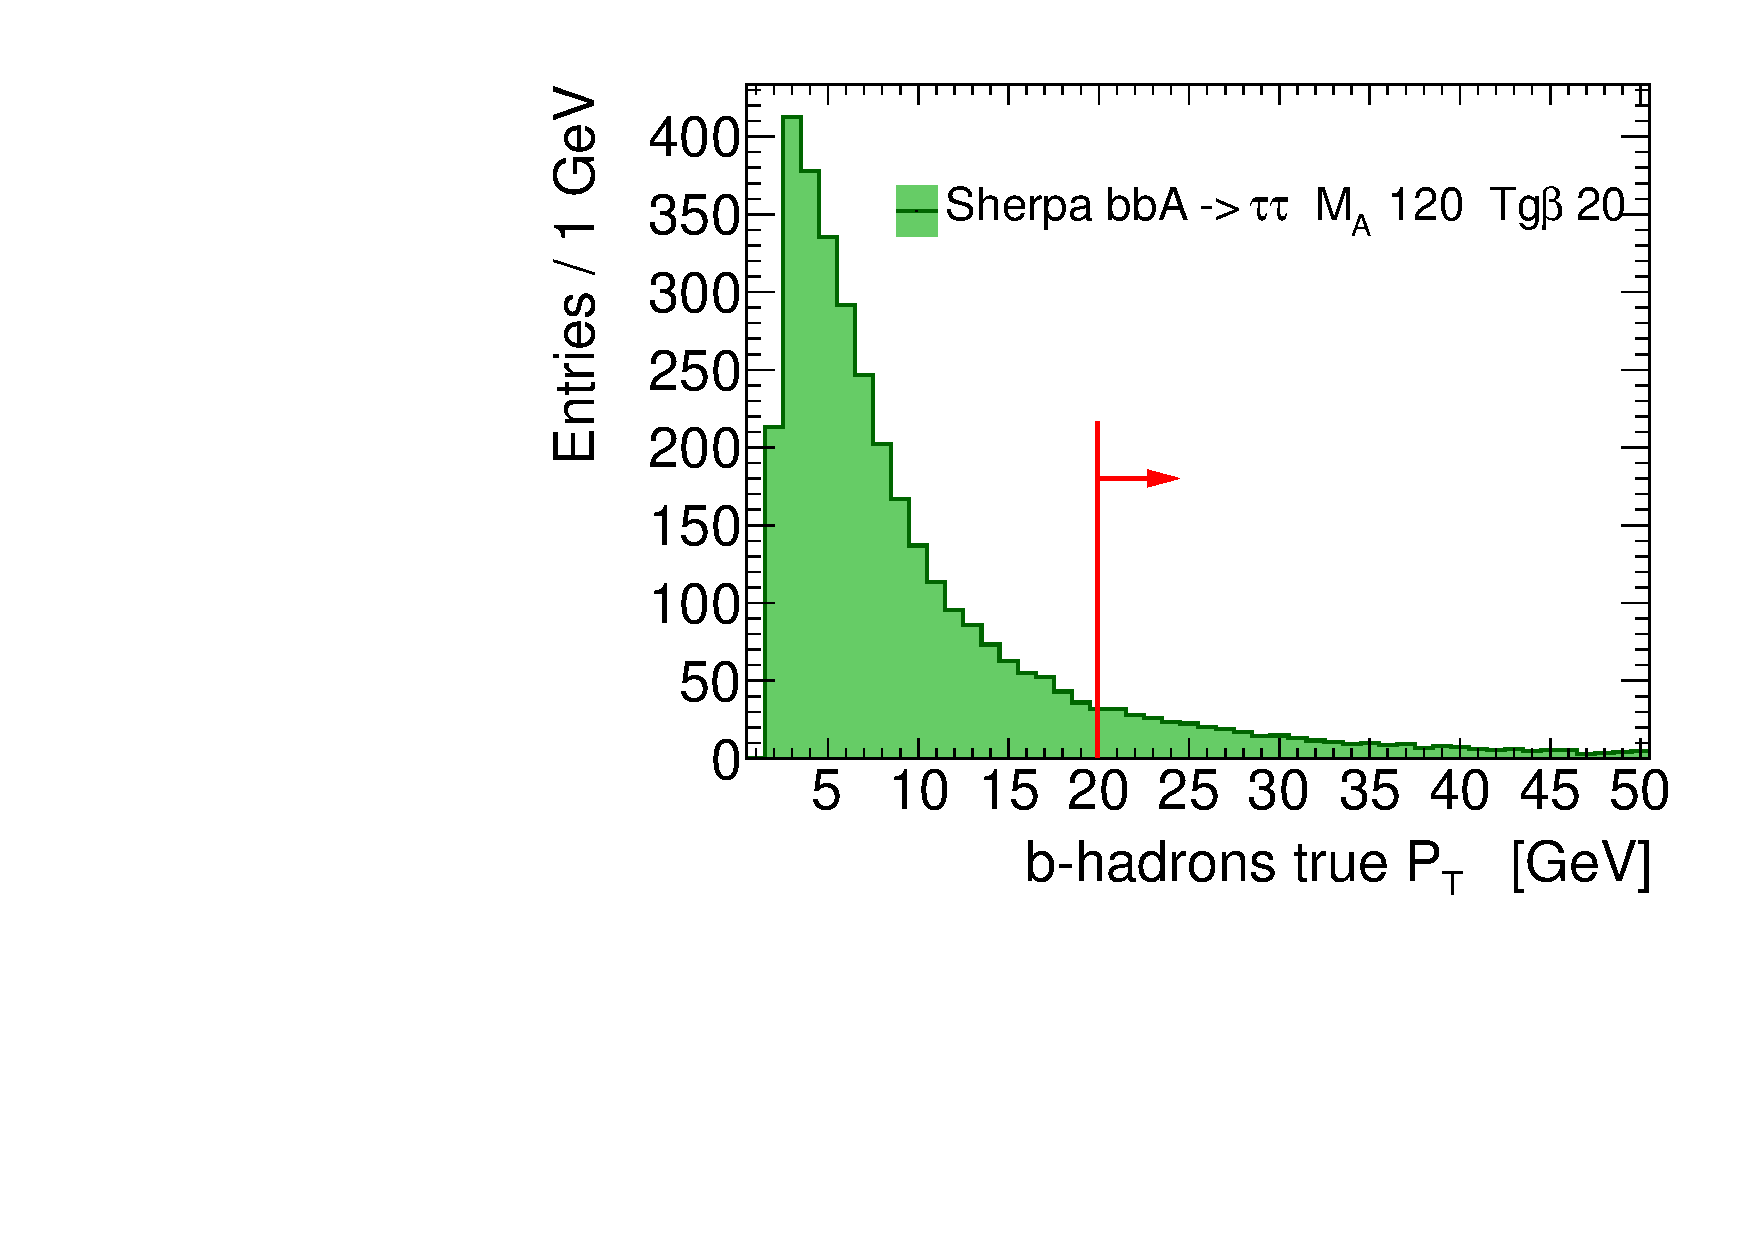
\includegraphics[width=0.49\textwidth]{figure/trackjet/b_pt_distro2.pdf}
            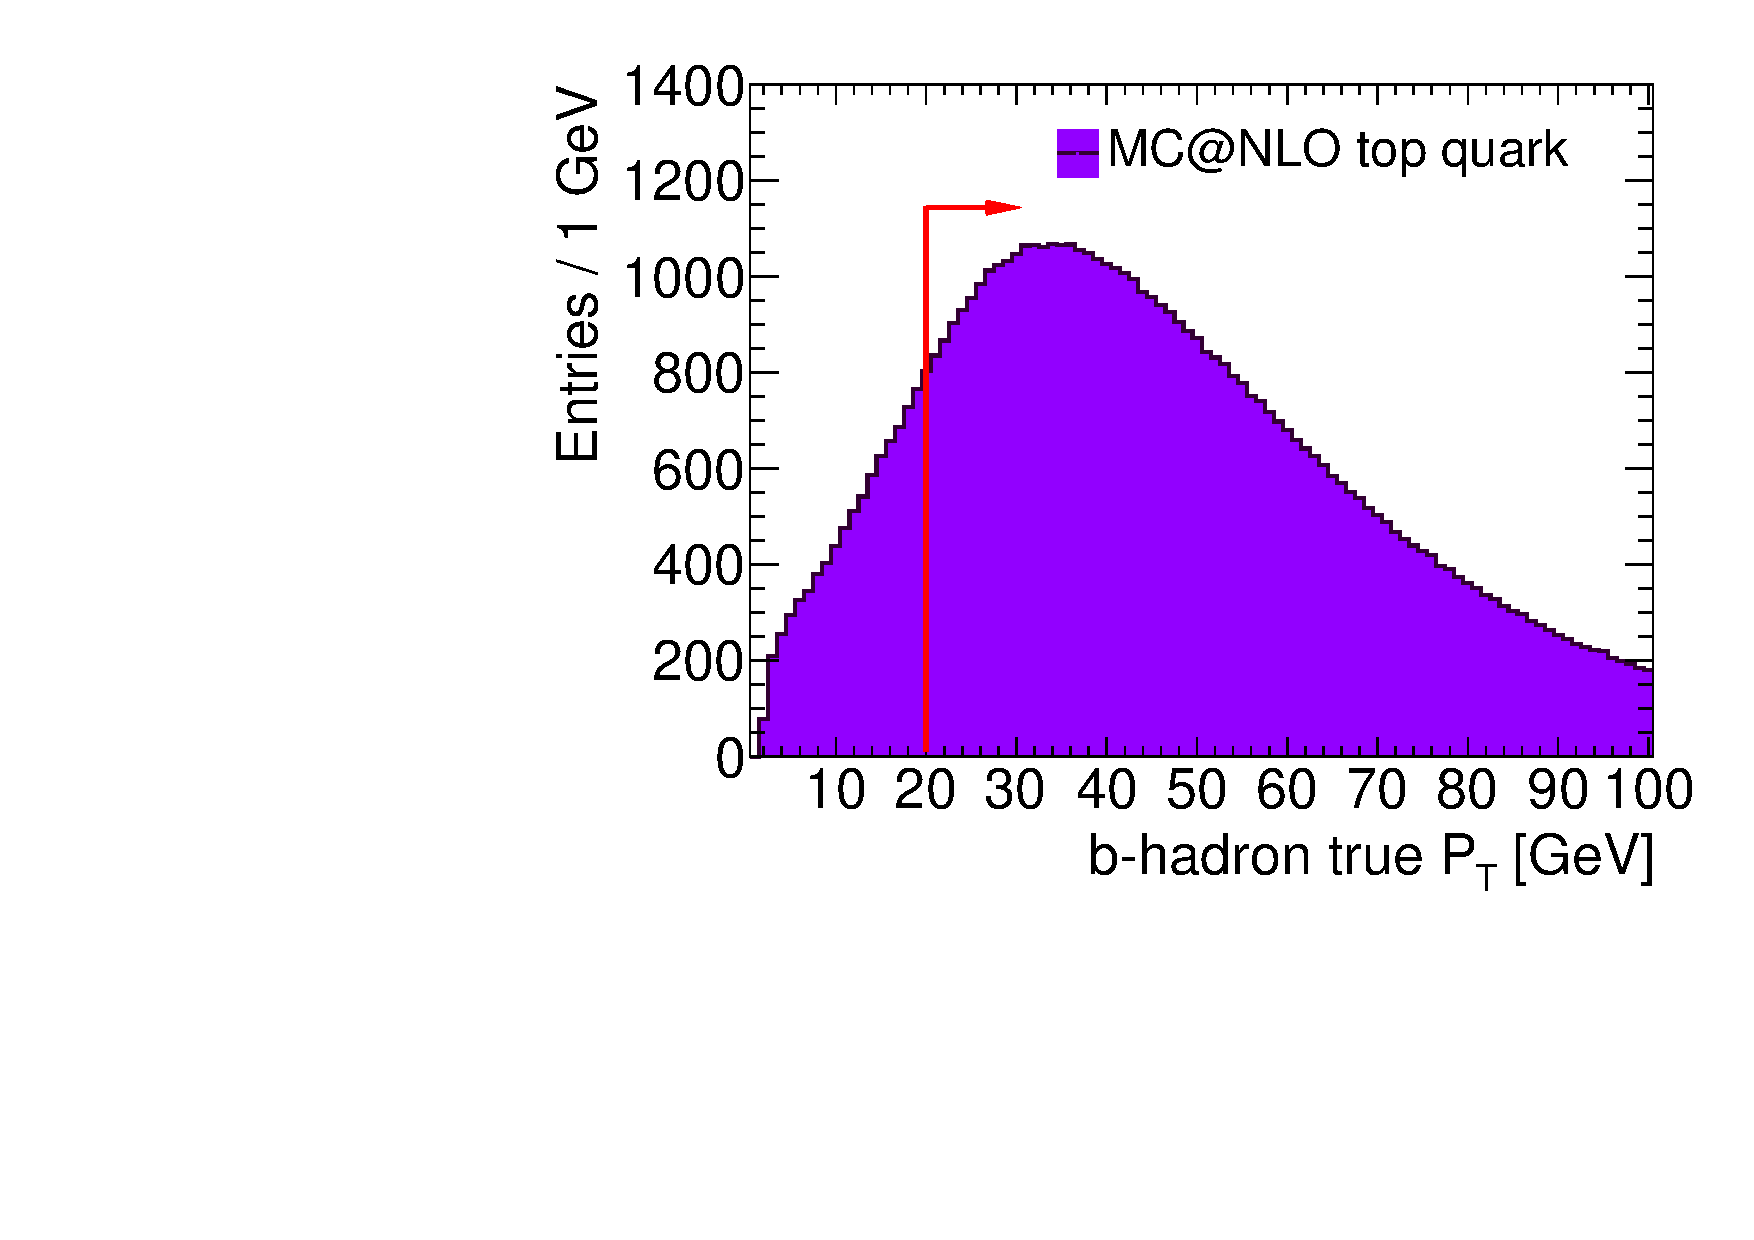
\includegraphics[width=0.49\textwidth]{figure/trackjet/top_pt_distro.pdf}

    \end{center}
    \caption{Simulated $\pt$ distribution of b-hadrons from b-quarks produced in association with the neutral MSSM Higgs boson 
	(left) 	and from b-quarks jet in  $\ttbar$ events (right). 
	The red line indicates the region in which the energy of the calorimeter jets can be calibrated.}
   \label{fig:bjetDistro}
\end{figure}


In the search for the neutral MSSM Higgs bosons, as described in chapter~\ref{chap:anal}, the selected events are categorized 
in two categories based on the presence or the absence of a b-tagged jet in the event. The b-tagged event category 
is optimized for the selection of Higgs bosons produced in association with b-quarks. Figure~\ref{fig:bjetDistro} shows a comparison 
between the $\pt$ spectra of simulated b-hadron (hadrons containing a b-quark) in $pp\rightarrow b(b)\,A/h/H$ process  and in $\ttbar$ events.
The signal contains  b-hadrons with relatively low transverse momenta, imposing a  major challenge 
for the analysis of the b-tagged event category. Due to the high amount of pileup and ambient energy density in the events, 
the energy of the calorimeter jets with $\pt<20$~GeV is not calibrated (see chapter~\ref{chap:obj}), the jet recostruction performance 
and related systematic uncertainties are not evaluated for these jets. The reconstruction of calorimeter jets in the $pp\rightarrow b(b)\,A/h/H$ 
signal production process is therefore not optimal and represent the major source of the sensitivity losses 
in the b-tagged event category.
An additional challege of the presented search is the worsening of the  b-tagging performance for jets with low transverse momenta. 
The efficiency obtained with the $MV1$ tagger decreases  rapidly  with jet $\pt$, reaching a minimum of 50\% at 
20~GeV for the tagging point with $\epsilon_b^{\ttbar}=70$\%~\cite{BtaggingScaleFactors,BtaggingScaleFactorsNew}.

The performance of the jet reconstruction for  low transverse momenta may be improved by introducing \emph{track-based} jets (in the following track-jets)
in repleacement to the commonly used calorimeter jets.
Track-jets are reconstructed with the anti-kt algorithm by  clustering inner detector tracks.
Conversely to calorimeter clusters, tracks have associated impact parameter informations and  track-jets can be reconstructed
with tracks originating from the same ineteraction point, making their reconstruction very robust against the impact of pile-up.

%%%%%% Definition of Track-jets %%%%%%%%%%%
Track-jets are built by the \emph{TrackZTool} reconstruction software which runs the anti-kt clustering 
algorithm on a subset of user-defined tracks.
For the purposes of this thesis track-jets are reconstructed  from tracks satisfying  the following
quality selection criteria:
\begin{itemize}
\item The track should be associated to the primary vertex (PV), \\$|z_{track} - z_{PV}| < 2$~mm, where $z_{track}$ and $z_{PV}$ are
 the absolute $z$ coordinate of the track and of the primary vertex, respectively.
 
\item The track is required to point to the PV in the plane  containing the beam axis by 
	$|z_{PV} \cdot sin(\theta)| < 1.5$ mm, where $\theta$ is the angle between the track and the beam axis.

\item The distance of minimum approach of the track to the  primary vertex  
in the plane orthogonal to the beam axis is required to be $d_{PV} < 1.5$ mm.


\item At least one pixel hit and at least 6 SCT hits (including SCT holes) should be detected for each track.

\item A  b-layer hit should be present if the b-layer module passed by the track was active.

\item The pseudorapidity of the track is required to be $|\eta| < 2.5$, corresponding to the coverage of the inner detector.

\item The track transverse momentum should be $\pt > 300 $~MeV to ensure a low track fake rate.

\end{itemize}
A track-jet is seeded by a cluster of at least two tracks which satisfy the above selection criteria, 
the sum of the transverse momenta of all associated tracks is required to be $\sum_ip_{T,i} > 2$ GeV.
It has been shown that the above selection criteria, together with a maximum cone size for clustering of 
$\Delta R = 0.6$, give the best compromise between the power of rejecting  fake tracks and the b-hadron reconstruction efficiency.
%to control "fakes" i.e. 
%tracks from random association of hits or badly reconstructed tracks, and b-hadron reconstruction efficiency.
%%%%%%% Definition of the Samples %%%%%%%%%%%%%%
Several simulation samples have been produced to study the performance of the track-jets reconstruction and of the b-tagging procedure
applied to these jets.
Table~\ref{tab:tackjetSample}  gives a list of the produced samples along with the type of studied performed with them.

\begin{table}[tp]
	\caption{Monte Carlo simulation samples.}  %%%%%da fare meglio !!!!!!!!!!!!!!!!!!!!!!!!!!!!!!!!!!!!!!
	\vspace{3mm}
\centering
	\begin{tabular}{l c c}
	\hline
	\hline
	Process		&	MC Generator 	& Purpose				\\
	\hline
	Minimum bias	& Pythia		& Systematics study 			\\
	$b\bar{b}$ 	& Alpgen		& Performance for low $\pt$ b-tagging 	\\
	$\Ztautau$ 	& Pythia		& Impact on the MSSM Higgs search 	\\
	$\ttbar$	& MC@NLO		& Impact on the MSSM Higgs search\\
	MSSM $bb/A/h/H$ & Sherpa		& Impact on the MSSM Higgs search \\ 
	\hline
	\hline
	\end{tabular}
	\label{tab:tackjetSample}
\end{table}
	

B-tagging has never been tested before on track-jets, in section~\ref{sec:tj_perf} the first study of b-tagging over track-jets 
performances is reported. 


%\subsection{Motivation}
%\subsection{Definition of Track-jet}
\section[Performance of the Track-based Jets]{Performance of the Track-based Jets Reconstruction and b-tagging}\label{sec:tj_perf}
%\subsection{B-tagging Performance}
\subsection{Track-based Jets Reconstruction}
Many analysis could profit from an enhanced b-jet reconstruction efficiency at low values of $\pt$. 
The studies presented in this section are aimed at comparing the  performance of the b-jet reconstruction 
efficiency and the common b-tagging algorithm for the calorimeter and track-based jets, focusing in particular on jets 
with low transverse momenta.
%Due to the high precision of the inner detector track-jets are robust against 
%pileup and is possible possible to reconstruct them up to very low transverse momentum,
%if they are used for the only purpose of b-tagging then calibration is also not needed,
%however, 

Even tough the track-jets are more robust against  pile-up effects, which is the main reason for 
not use calorimeter jet at low transverse momenta, they contain only the charged fraction of the jet, 
while the neutral jet component is lost.
According to isospin invariance the expected charged fraction in a jet amounts to roughly $2/3$ of the total energy.
The track-jet momentum is therefore shifted accordingly and there is a larger 
uncertainty on its measured direction. Figure~\ref{fig:residuals} shows the 
distribution of transverse momentum residual $p_{T\,true} - p_{T\,jet}$ relative to the truth value $p_{T\,true}$ 
from \emph{truth-jet} (see chapter~\ref{chap:obj}) separately for calorimeter and track-jets.
Here truth-jets are matched with reconstructed jets within a cone of size  $\Delta R = 0.4$\footnote{jet splitting effects are resolved by matching with the nearest jet}.
As expected the track-jets energy is shifted from zero. This effect can be critical for most of the b-tagging algorithms 
since the likelihood functions used for decision making are derived separately for different region
of jets $\pt$ and pseudorapidity. A dedicated track-jets calibration of b-tagging algorithm is auspucable 
for  future application of b-tagging on these jets.
%in based on 
%like for example JetFitter, which
%strongly rely on the measurement of the jet axis and jet $\pt$.

\begin{figure}[tp]
\centering
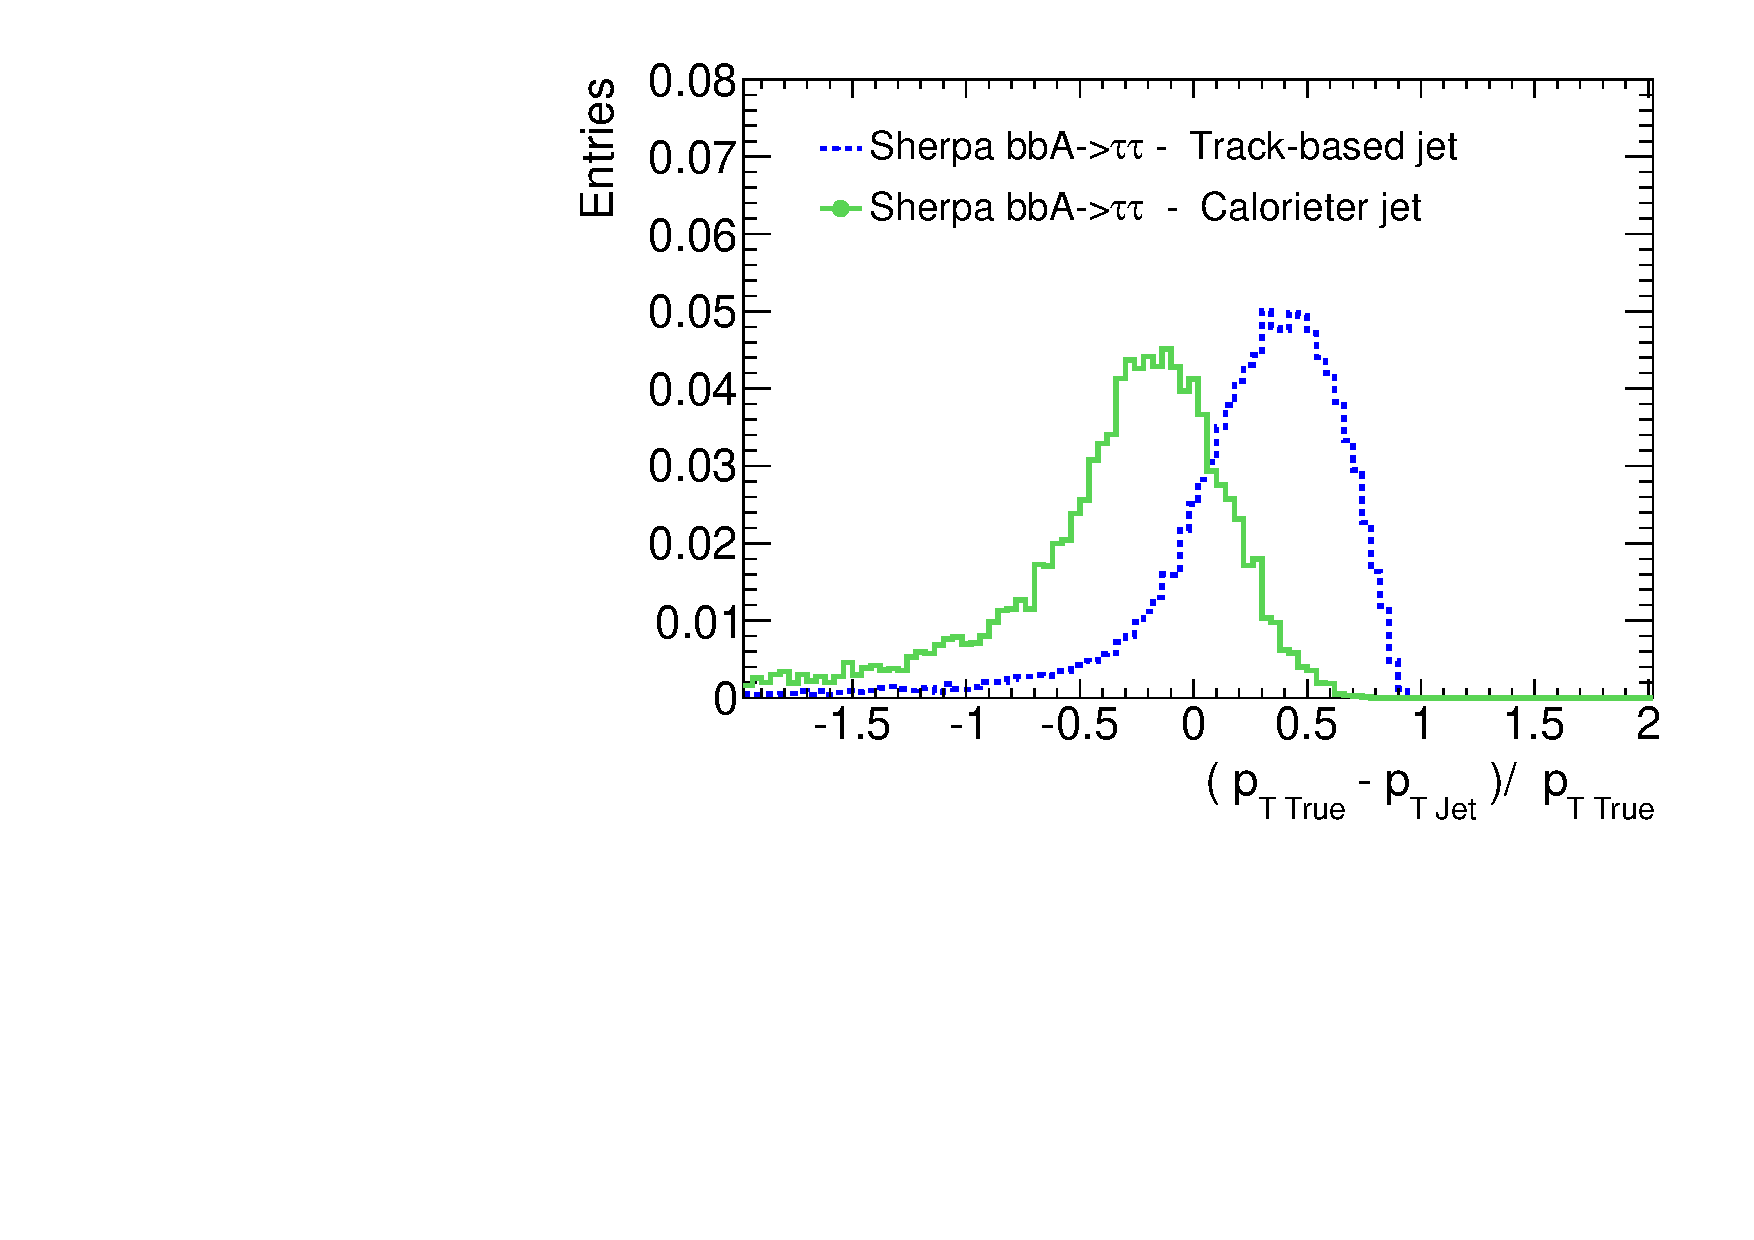
\includegraphics[width=0.7\textwidth]{figure/trackjet/residuals2.pdf}
\caption{Distribution of transverse momentum residuals relative to the true value $P_{T \, true}$,
shown separately for the calorimeter and track-jets.}
\label{fig:residuals}
\end{figure}    

To compare the performance of calorimeter and track-jet reconstruction, an anti-kt algorithm with cone size of $\Delta R = 0.4$ is chosen.
If the angular distance between the reconstructed jets and a simulated b-hadron in the event is $\Delta R  < 0.3$,
this jet is said to \emph{match} with a b-hadron. 
 b-hadron \emph{Reconstruction efficiency} is then defined as the ratio between the number of matched b-hadrons
and the total number of b-hadrons within inner detector acceptance. Figure~\ref{fig:recoEff} shows the  
b-hadron reconstruction efficiency for the calorimeter and track-jets. The latter exhibit a higher reconstruction efficiency at low 
transverse momenta due to their robustness against  pile-up effects.
\begin{figure}[tp]
\centering
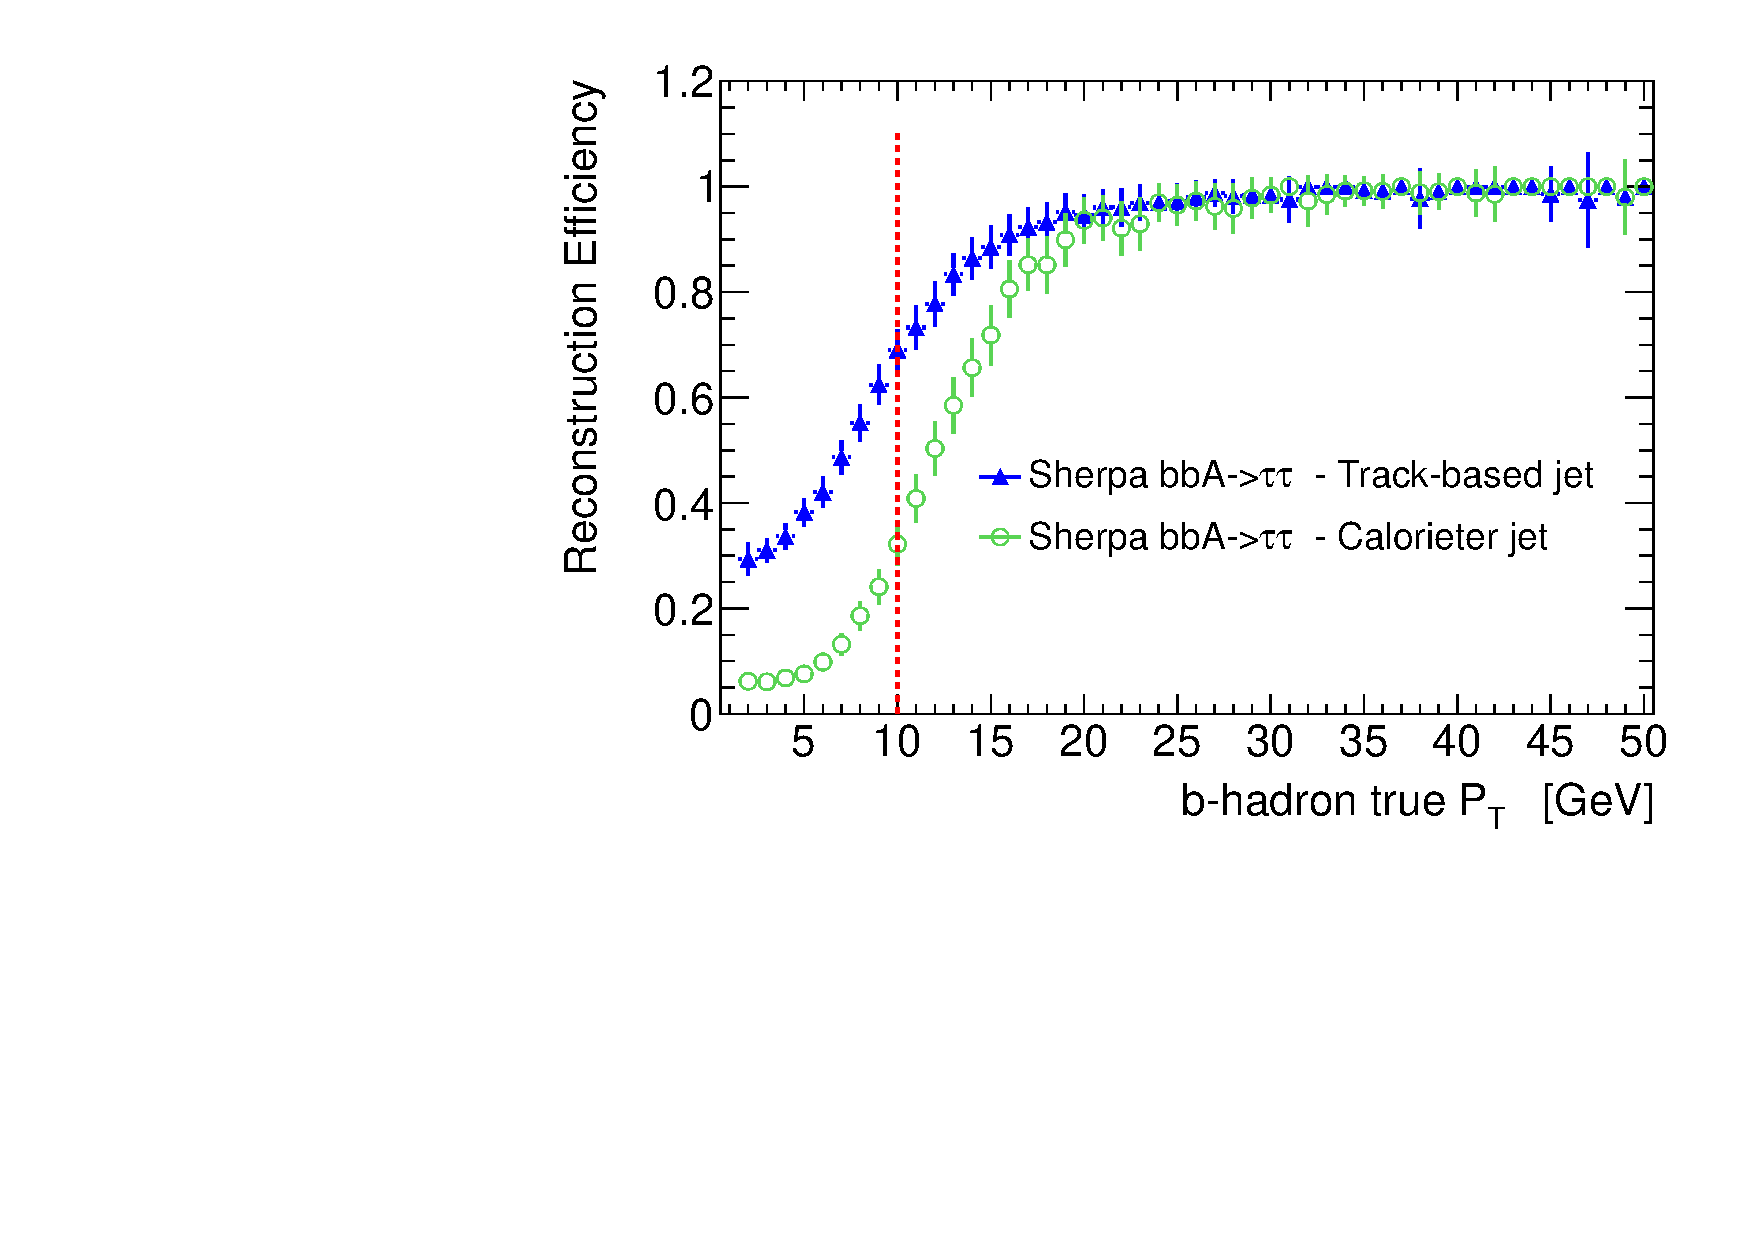
\includegraphics[width=0.7\textwidth]{figure/trackjet/rec_eff2.pdf}
\caption{b-hadron reconstruction efficiency for track-jet and calorimeter jets  as a 
function of the true b-hadron $\pt$. Note that calorimeter  and track-based jet are required to have at 
reconstruction level $\pt > 7$ and 2 GeV, respectively. A fair comparison in this plot is only possible
for $\pt > 10$~GeV.}
\label{fig:recoEff}
\end{figure}    

\subsection{B-tagging with Track-Based Jets}
Performance of the b-tagging algorithms is usually described in terms of the b-tagging
efficiency and rejection power against misidentified jets. The \emph{b-tagging efficiency} is the fraction of jets
matched to a true b-hadron which pass a given tagging selection criteria, i.e. which are \emph{b-tagged}.
The \emph{rejection power} is the inverse of the misidentification rate, i.e. the inverse of the fraction 
of jets which are not matched with a b-hadron or c-hadron, but are b-tagged. 
Figure~\ref{fig:eff_rej} shows the rejection power as a function of the b-tagging efficiency for various b-tagging 
algorithms applied on track-jets and calorimeter jets separately. Figure~\ref{fig:rej_pt}  shows the rejection power as a function of jet $\pt$ for the
b-tagging working point  which gives 50\% b-tagging efficiency, calorimeter and track-based jet are shown separately. Mistagging rate is rapidly increasing
for low transverse momentum jets due to increasing particle multiple scattering and secondary interactions in the material,
revealing the necessity of a dedicated b-tagging algorithm for low $\pt$ jets.

\begin{figure}[!tp]
\centering
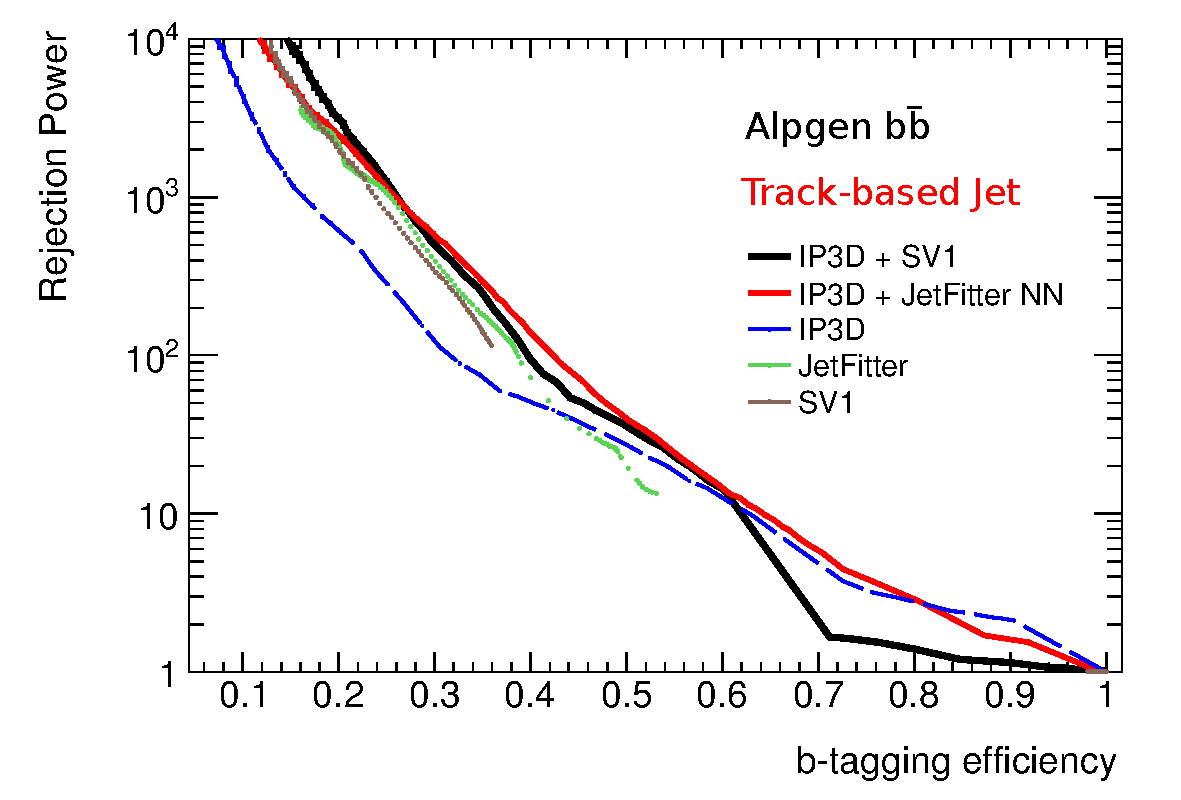
\includegraphics[width=0.7\textwidth]{figure/trackjet/std_eff_rej2.pdf}
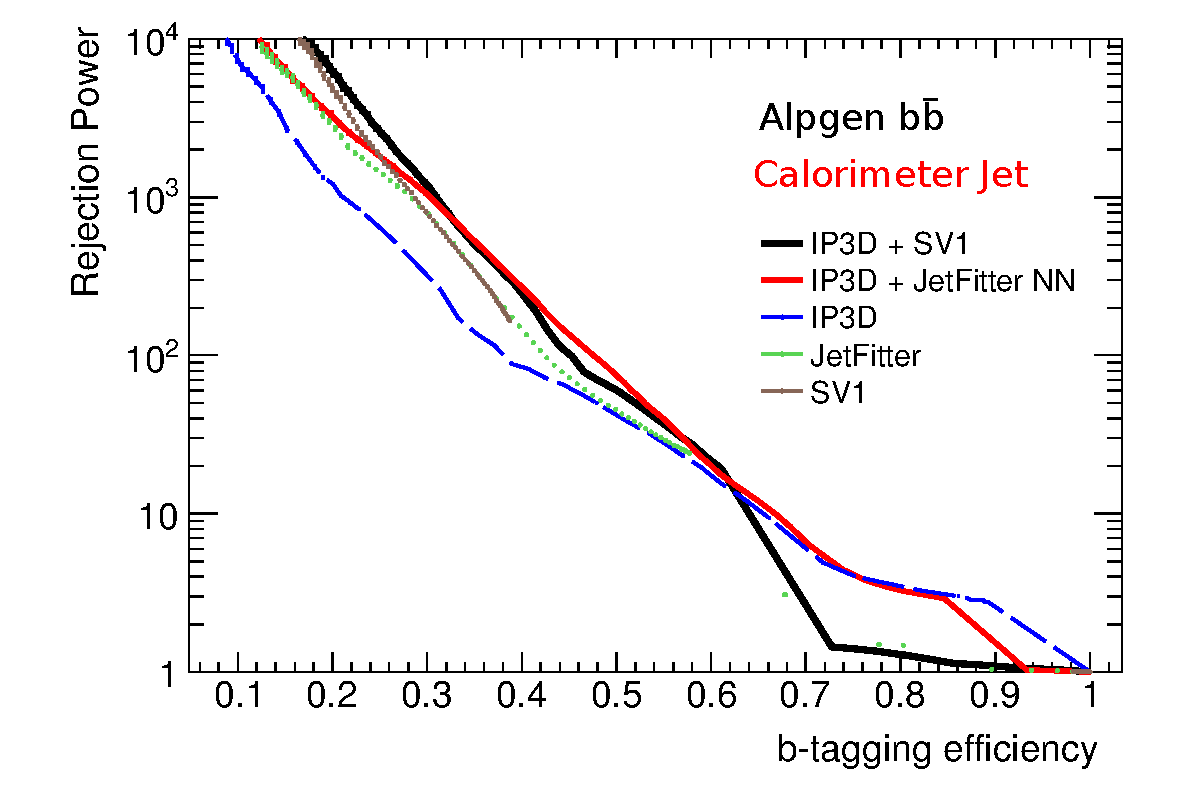
\includegraphics[width=0.7\textwidth]{figure/trackjet/std_cal_eff_rej2.pdf}
\caption{Rejection power as a function of the b-tagging efficiency for different b-tagging algorithm applied
	 on track-jets (top) and on calorimeter jet (bottom) for simulated $b\bar{b}$ events.}
\label{fig:eff_rej}
\end{figure}    

\begin{figure}[!tp]
\centering
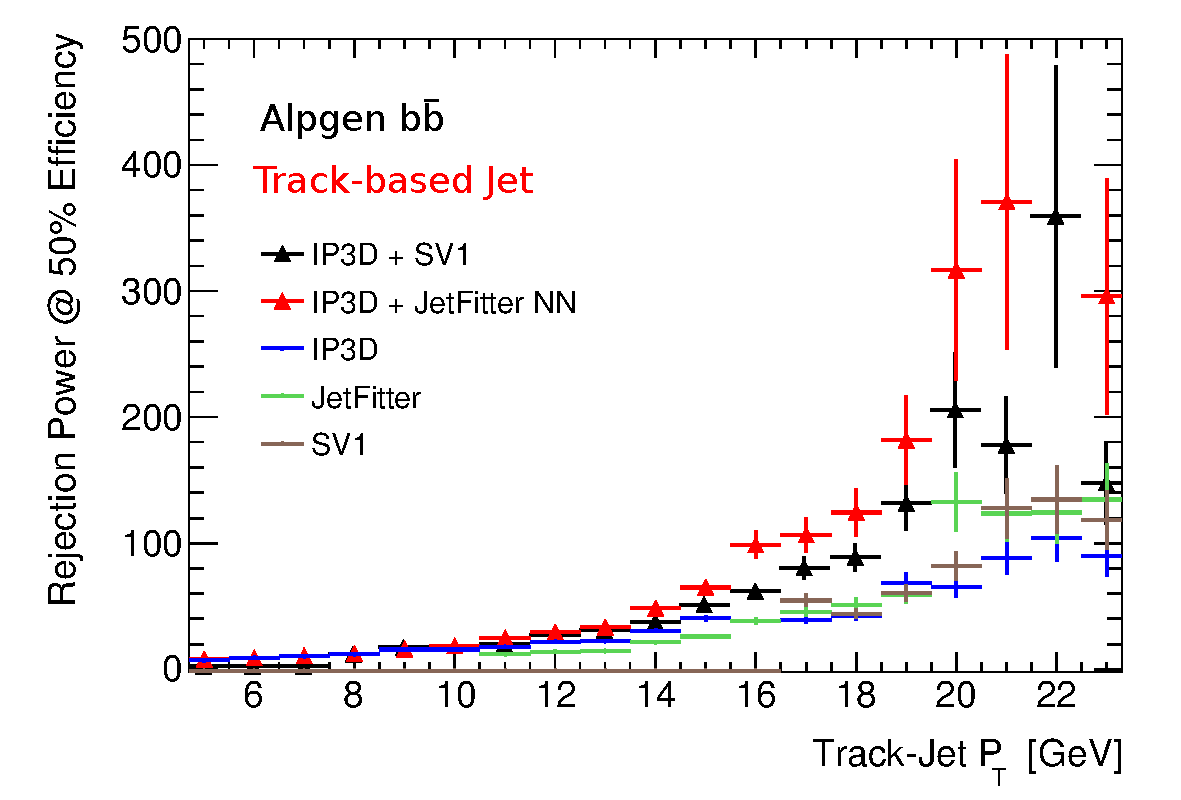
\includegraphics[width=0.7\textwidth]{figure/trackjet/std_rej_pt2.pdf}
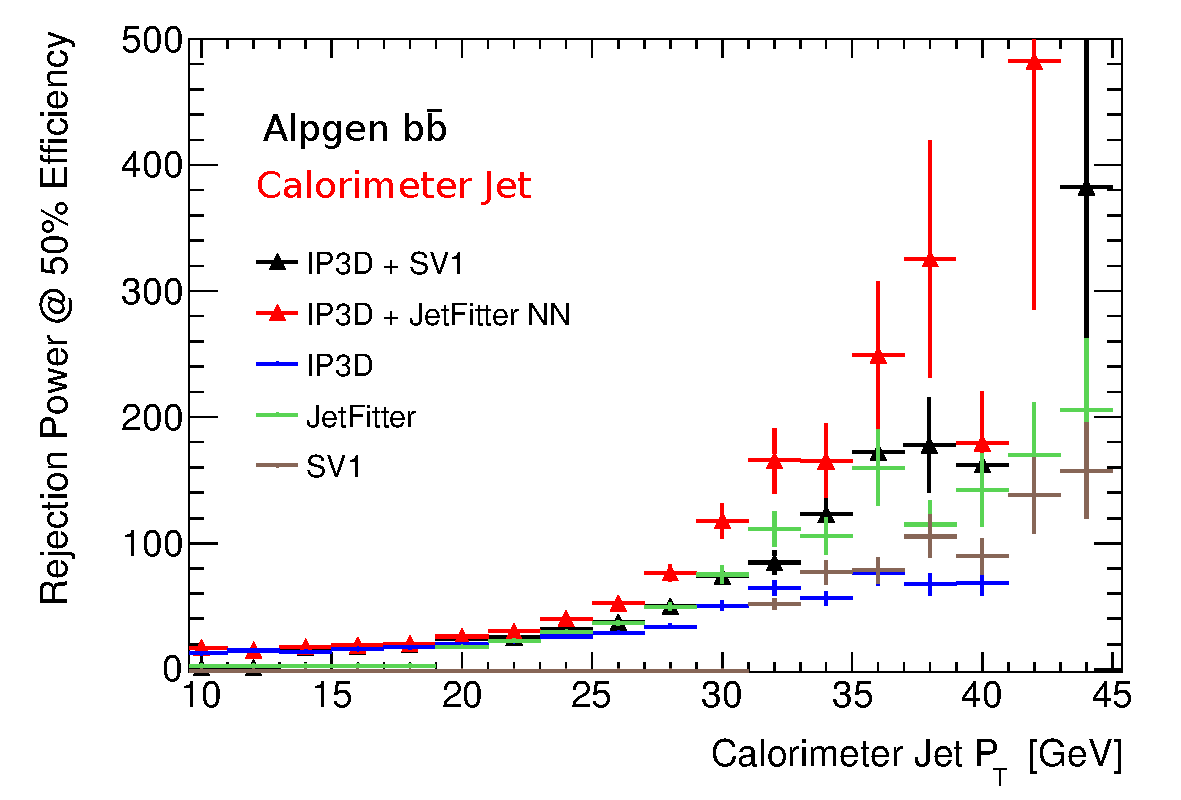
\includegraphics[width=0.7\textwidth]{figure/trackjet/std_cal_rej_pt2.pdf}
\caption{Rejection power as a function of the jet transverse momentum for the b-agging 
	working point whita  50\% b-tagging efficiency at that $\pt$ value, track-jet (top) and calorimeter jet (bottom) are
	shown separately. Results are obtained using simulated $b\bar{b}$ events
	and shown for several b-tagging algorithms.}
\label{fig:rej_pt}
\end{figure}    

\begin{figure}[!tp]
\centering
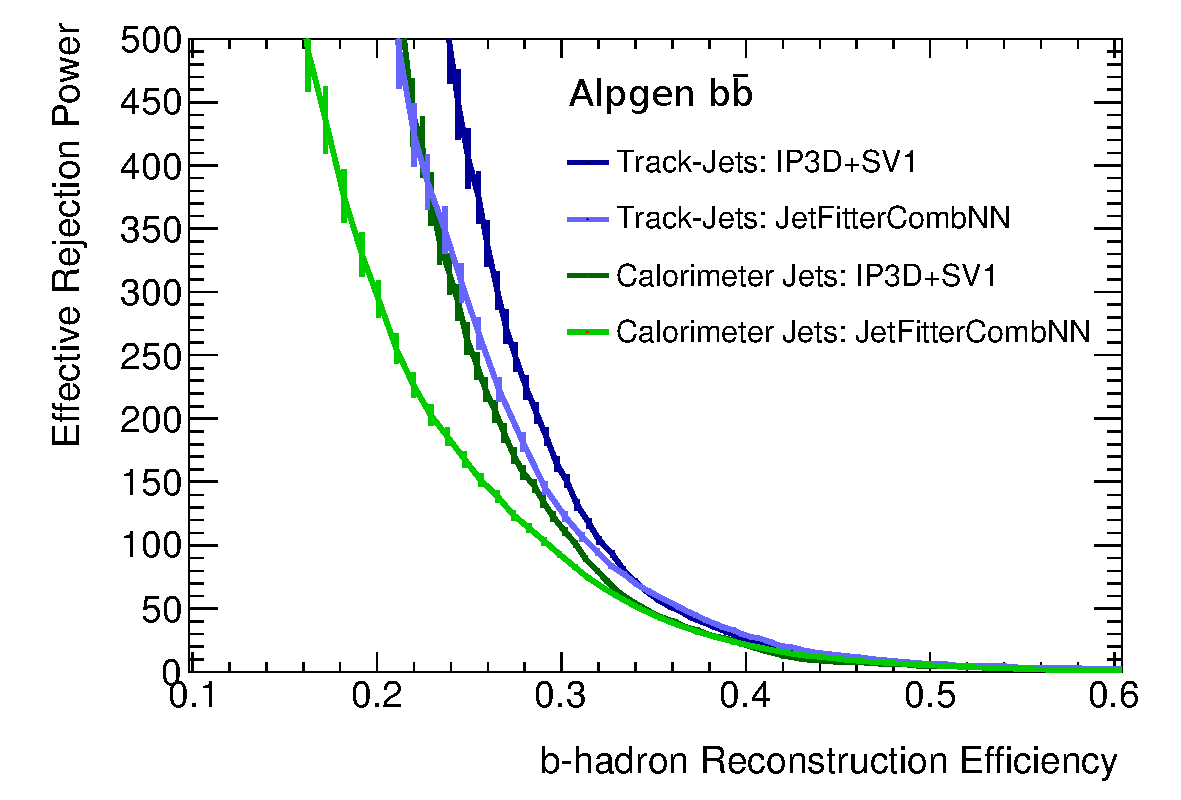
\includegraphics[width=0.7\textwidth]{figure/trackjet/eff_real_rej_mod2.pdf}
\caption{Effective rejection as a function of b-hadron reconstruction efficiency, track-jet and calo jets are
	compared for two different ATLAS tagging algorithms. Track-jets are selected in the transverse momentum range 
	between 4 and 33 GeV, while calojets between 8 and 50 GeV.}
\label{fig:cj_tj}
\end{figure}    

The described rejection power and b-tagging efficiency cannot serve for a fair  comparison of the track-based and calorimeter jets.
The latter can be reconstructed even if there are no associated tracks to them, in which case any b-tagging algorithm will most likely fail.
The distribution of the rejection power is therefore altered by such jets. It is instead convenient to introduce 
the: \emph{effective rejection power}, which is the inverse of the number of mistagged jets per event. 
Figure~\ref{fig:cj_tj} shows the effective rejection power as a function of the b-hadron reconstruction efficiency, for 
calorimeter and track-based jets. For a given b-hadron reconstruction efficiency,
a higer effective rejection of mistagged jets can be achieved by track-jets.
For a fair comparison with calojets the track-jets in Figure~\ref{fig:cj_tj} are selected in the transverse 
momentum range between 4 and 33 GeV, while the transverse momentum of calorimeter jets 
ranges from 8 to 50 GeV. The introduced $\pt$-thresholds corresponds in averange to the same $\pt$ range, 
Figure~\ref{fig:residuals} is only valid for low $\pt$ jets  and the fraction of undetected 
momentum from neutral jet component  approaches 1/3 for higher $\pt$ track-jets.
In conclusion, for jets with low transverse momentum the track-jets provide a higher 
b-hadron reconstruction efficiency than calorimeter jets and are more suitable  for 
low $\pt$ b-tagging.

\subsection{ Use of Track-jets for the MSSM Higgs Boson Search} % A new Hope
The impact of the track-jets selection on the search for the neutral MSSM Higgs bosons is tested in a 
preliminary study and reported in the  following. 
Common selection criteria,\footnote{This study has not been updated with the latest version of the object reconstruction 
		selections and corrections, a difference of the order of 10\% is expected with respect the 
	    	numbers in table~\ref{tab:eventsel:btag}.},
as defined in in Section~\ref{sec:presel}, are applied to simulated signal and background samples with the following modifications
concerning the jets on which b-tagging procedure is applied (taggable jets):
\begin{itemize}
\item Calorimeter jets should have $|\eta| < 2.5$ and $20 < \pt < 50$ GeV.
\item Track-jets should have $|\eta| < 2.5$ and $5 < \pt < 33$ GeV.
\item The b-tagging algorithm applied on the above jets is "IP3D+SV1" at a 
	working point with a $\epsilon_b^{\ttbar}=70$\% tagging efficiency.
%this correspond to the same
%  	range as for calojets above, figure~\ref{fig:residuals} in fact is only valid for low $\pt$ jets
%	and the fraction of momentum lost  1/3 for high $\pt$ track-jets. 
\end{itemize}
The minimum transverse momentum for which calorimeter jet are calibrated is 20~GeV, track-jets instead can 
safely access transverse momentum up to 5~GeV.
The event yields expected for the $pp \rightarrow b(b)A/h/H$ signal process, $\Ztautau$  and $\ttbar$ background processes
(the two most important background contributions in the b-taged event category) 
are reported in Table~\ref{tab:tj_cj}. The yields are  normalized to an integrated luminosity of $1 ~ fb^{-1}$.
In addition to the event yields after the common selection stage other b-tagging related selection
requirements  are applied to study the impact of the replacement of calorimeter with track-based jets.
As expected, after requiring exactly one b-tagged jet, the track-jets reconstruction 
results in a higher signal efficiency with a relatively similar rejection (10\% higher) of top quark 
background compared to calorimeter-based jet reconstruction.
However, lower transverse momentum threshold for the  track-jets implies higher mistagging rates,
as can be seen from an increase of $\Ztautau$ background. This may also lead to a strong contamination of the 
QCD multi-jet background, even tough this is a minor background contribution in b-taged event category.

\begin{table}[tp]
	\caption{Event yield for the signal and dominant background processes after different event selection requirements.
	The yields are shown separately for the calorimeter and the  track-based jet reconstruction.
	The Higgs boson produced in association with b-quarks is simulated for  $\tan\beta=20$ and $m_A=150$~GeV. The yields
		are normalized to an integrated luminosity of $1 ~ fb^{-1}$.}
	\vspace{3mm}

	\begin{footnotesize}
	\begin{tabular}{p{3.0cm} |c c| c c| c c }
	\hline
	\hline\\ 
Selection 	& 	\multicolumn{2}{|c|}{Signal $bbA/H/h$ }	&\multicolumn{2}{c|}{$\Ztautau$}	& \multicolumn{2}{c}{$\ttbar$}	\\
	[0.5cm]
%	\noalign{\smallskip}
	\hline
Common Selection	&	\multicolumn{2}{|c|}{$127.2 \pm 2.2$} &\multicolumn{2}{c|}{$3017 \pm 8$} &\multicolumn{2}{c}{$2066 \pm 5$} \\[0.5cm]
			&	Calo. jet		&	Track-jet &Calo. jet	&Track-jet	&Calo. jet	&Track-jet \\[0.5cm]
At least one taggable jet& $47.3 \pm0.8$	&$106.9 \pm1.8$	 &$1146 \pm3 $	&$2513 \pm 7$	&$1804 \pm 4$	&$2014 \pm 5$ \\[1cm]
Exactly one jet matched to a b-hadron& $18.4 \pm 0.3$ & $46.7 \pm 0.8$ & $4.5 \pm 0.3$	&$18.2 \pm 0.5$ 	&$1054 \pm 3$	&$959.1 \pm 2.3$  \\[1cm]
Exactly one b-tagged jet&	$10.2 \pm0.1$	&$21.0 \pm 0.6$	& $37.3 \pm 0.5$ &$107 \pm 1$ &$777 \pm 4$	&$630 \pm4$ \\[1cm]
	\hline
	\hline
	
	\end{tabular}
	\end{footnotesize}
	\label{tab:tj_cj}
\end{table}

In conclusion, the neutral MSSM Higgs boson search presented in the previous chapter may be improved if track-jet
reconstruction is applied instead of calorimeter based one.
The sensitivity\footnote{Note that the sensitivity is estimate according to the $s/\sqrt{b}$ ratio (where $s$ and 
$b$ are the signal and background yield respectively), considering a counting experiment without systematic uncertainties and 
with only two background processes, this corresponds to the maximal possible sensitivity achievable 
 with the current b-tagging performance.} 
to the signal can be improved in this event
category by about a factor two. However, to exploit the full power of this technique a dedicated calibration of the 
b-tagging algorithms is  needed for the track-jets. Additional improvements of the b-tagging algorithms 
for low $\pt$ b-jets are also desirable. Furthermore, 
systematic uncertainties of track-jet reconstruction need to be evaluated. A preliminary study, addressing some
 of the most important of such systematic uncertainies is reported in section~\ref{sec:trackjetsys}.
 
%\subsection{A Novel Technique for low-$\pt$ b-Tagging} % variable to enhance low pT b-tagging
%\textbf{this small paragraph will be added if I manage to access track-jets data on MDTRaid16}, 
%I just need to reproduce one plot which is missing.


\section{Systematic Uncertainties of Track-Jet Reconstruction}\label{sec:trackjetsys}

%why Energy scale...
%Uncertainty on physics observable related to track-jets due to MC mismodeling needs to be evaluated,
%uncertainty arises from non perfect modeling of track-jets direction, energy scale and reconstruction efficiency,
%
%There are several sources that may give contribution to systematic uncertainties on the energy scale of track-jet, those
%effects  are briefly summarized in what follows. 
%

%\subsection{Introduction to Track-jet Systematics}

There are several sources of systematic uncertainties of the track-jet reconstruction that may contribute to
the mismodeling of physics observables.  These effects  are briefly summarized in the following with an ephasis on 
uncertainties of the energy scale and reconstruction efficiency. %since they will have the biggest
%impact on any physics observable that may be interesting for us.

Uncertainty on the properties of simulated track-jets can arise from the Monte Carlo generator
configurations, depending on the particular choice of PDF and fragmentation functions, or details of the parton shower and underlying 
event modeling, which have a significant impact on physics objects with low transverse momentum. 
These uncertainties can be evaluated by means of a dedicated analysis with the Rivet package~\cite{RIVET}.
They depend on the particular  use of track-jets and need to be evaluated case by case.

Energy scale and resolution of single tracks is found to be very well modeled by simulation for tracks above
500 MeV \cite{IDperformance}. Thus, uncertainty on the track-jet energy scale and resolution that arise from the mismodeling of
the pattern recognition procedure are considered to be negligible. 

In a dense track environment  different tracks may share 
same hits, leading to a degradation of the track momentum resolution, fake tracks and losses of track reconstruction
efficiency. Mismodeling of the hit sharing among several tracks may in general affect the 
track-jet energy scale, resolution and reconstruction efficiency. 
Such effects has been studied in~\cite{JEStrack}, where energy scale uncertainties for  calorimeter jets is 
measured based on associated tracks. It has been shown that effects due to the merging of track hits are negligible 
for jets with $\pt < 300$~GeV.

Mismodeling of the inner detector material budget leads to the mismodeling of the 
to track reconstruction efficiency, which strongly affects also the track-jets reconstruction.
A methodology to estimate the uncertainty of the energy scale and reconstruction efficiency for track-jets due to the
mismodelling of the material budget is studied for the first time and presented in section~\ref{sec:trackExMat}.


\subsection{Material Budget Uncertainty on Track-Based Jets Reconstruction } \label{sec:trackExMat} %general description of the method
An obvious but rather inconvenient way to estimate the uncertainty due to the mismodeling of the 
inner detector material budget is to simulate the  Monte Carlo samples relevant for a given analysis 
using several different ID material budgets.
It can be shown that the mismodeling of material budget primarily influence the
track reconstruction efficiency (see section~\ref{sec:valid}). An alternative approach is therefore to
modify the track reconstruction efficiency in a given sample according to the corresponding uncertainty~\cite{IDMaterial,trackEff} and build 
track-jets from such  new collection of tracks.
A tool has been developed which randomly removes tracks according to the uncertainty on  reconstruction efficiency. 
The track-jets which are build from  this subset of tracks are called in the
following \emph{inefficient} track-jets. 

The standard and inefficient track-jets are compared in a simulated sample of minimum bias processes. 
A set of "isolated" track-jet with cone size $\Delta R = 0.4$ are selected, where the isolation 
means that no other track-jet should be reconstructed within an angular distance of $\Delta R = 1$. 
Inefficient track-jets are then matched with the original track-jet in the same event,
the matching fails if no inefficient track-jet is found within a cone of size $\Delta R = 0.8$ around
the original track-jet. The impact of tracking inefficiency on track-jet energy scale and reconstruction
efficiency is presented respectively in Figure~\ref{fig:inef_tj_std_scale} and \ref{fig:inef_tj_std_eff}$\,$. These 
results are based on the current knowledge of the inner detector material budget~\cite{IDMaterial}. 
Since track-jets are required to have at least two tracks at reconstruction level, if a track 
is lost that jet  cannot be reconstructed anylonger, therefore for track-jet with two tracks 
the only effect is a loss of reconstruction efficiency. For track-jets with low transverse momentum, uncertainty on the material budget 
translates into an energy scale shift of 2-4\% and in a reduction of the mean number of tracks.

This method can only simulate excess of material (reduced track efficiency) but not a lack of material
(increased track efficiency). However, for the latter case a symilar, symmetric impact is expected.

\begin{figure}[tp]
\centering
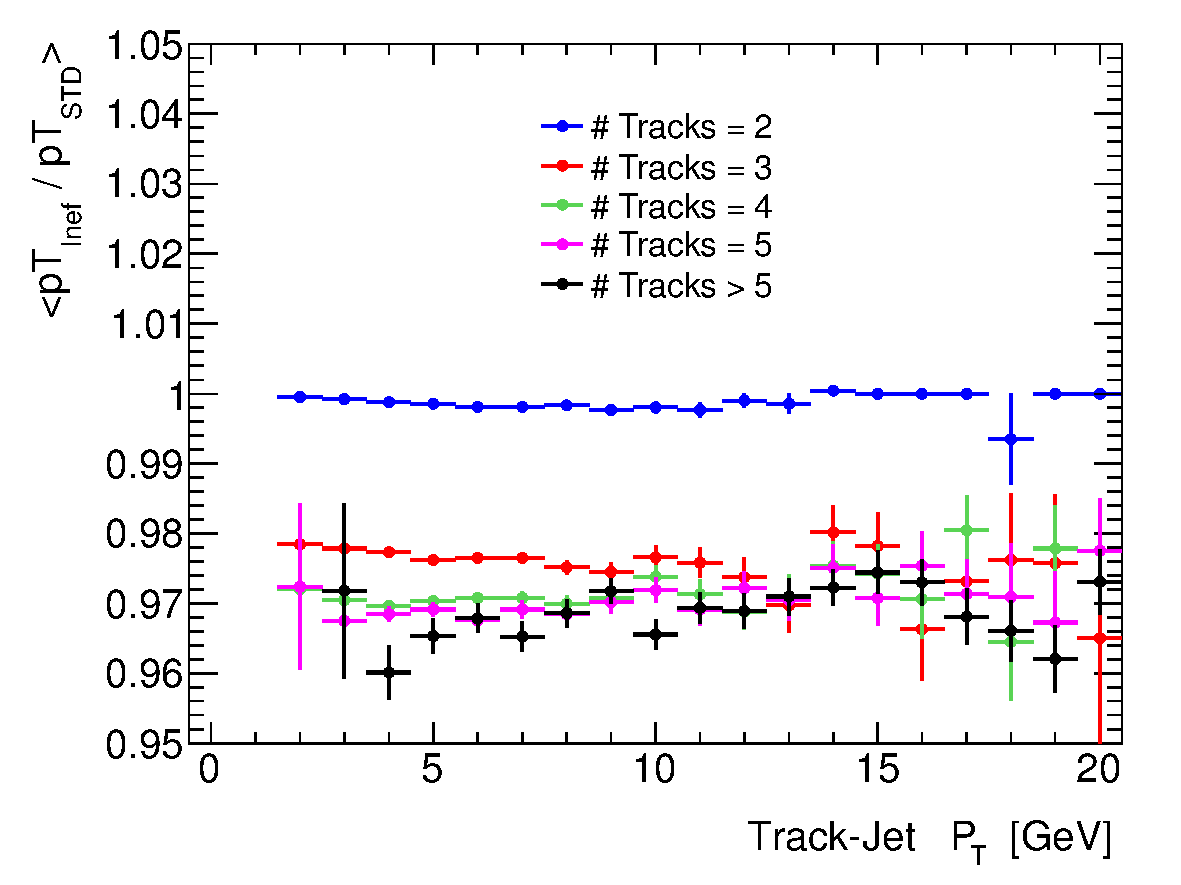
\includegraphics[width=0.7\textwidth]{figure/trackjet/T7/Sys_pt_nTrack2.pdf} 
\caption{Inefficienct track-jets are matched with standard track-jets. The average transverse momenta of the inefficient track-jet $p_{T \, inef}$
	relative to the corresponding standard track-jet $p_{T \, std}$ is shown as a function of the 
	$\pt$ and number of associated tracks of the standard track-jet.}

\label{fig:inef_tj_std_scale}
\end{figure}    


\begin{figure}[tp]
\centering
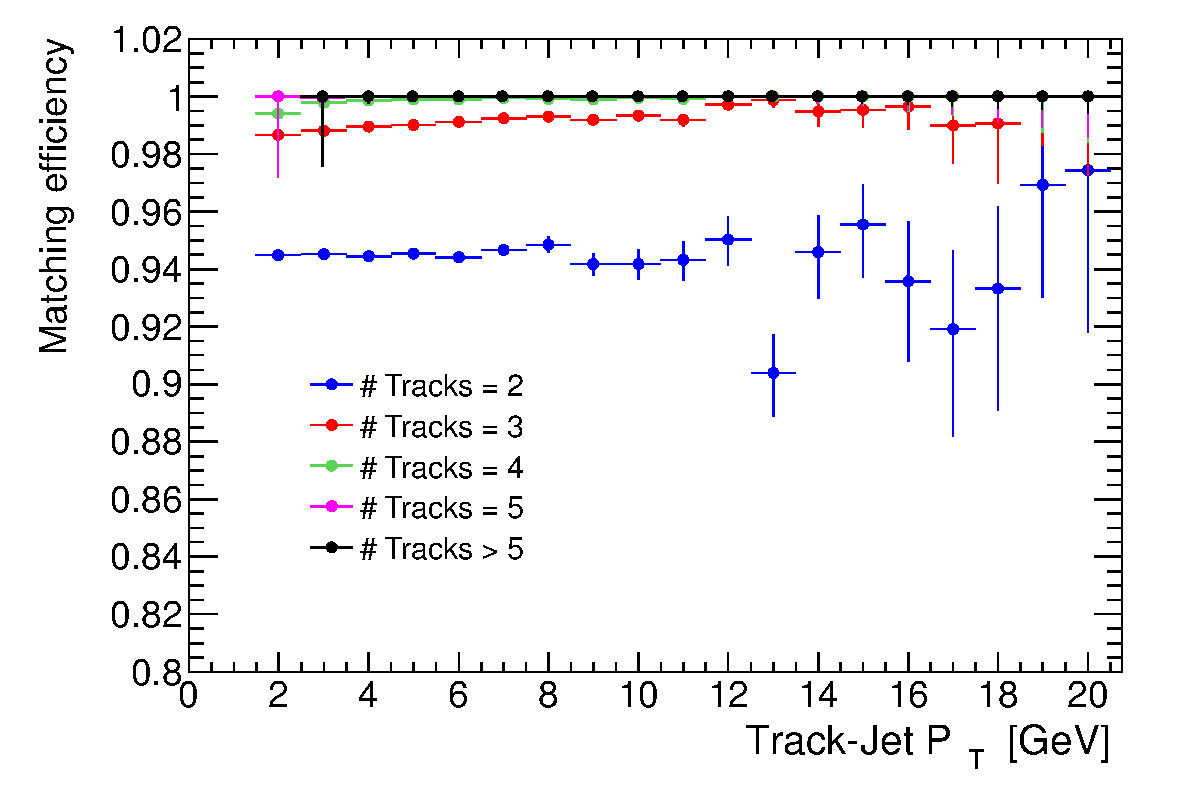
\includegraphics[width=0.7\textwidth]{figure/trackjet/T7/Sys_eff_n2.pdf}
\caption{Inefficient track-jets are matched with standard track-jets. The matching efficiency is shown as a function of 
	the $\pt$ and number of tracks associated with the  standard track-jet.}

\label{fig:inef_tj_std_eff}
\end{figure}    


\subsection{Validation of the Track Subtraction Method} %confermo che l'effetto di Ex material e' solo efficiency
\label{sec:valid}
%effect on tracks of a 10% EX sample
The method described in section~\ref{sec:trackExMat} depends strongly on the assumption that 
%the main effect of 
% material budget mismodeling is a loss or gain in track reconstruction efficiency, meaning that 
hadronic secondary interactions within the inner detector material  lead manly to the loss of 
some tracks and only in a marginal way to a decrease of the track quality. As a consequence, the misodeling 
of the material budget is expected to influence mainly the track reconstruction efficiency.
%this is equivalent to say that the quality selection on tracks are robust enough.
In this section, the impact  of the  material budget uncertainty on the track momentum resolution 
and fake rate is evaluated using a simulated  sample of minimum bias events, in which additional material 
is added to the ID increasing uniformly of 10\% the interaction length.  

For this study, the track selection is performed as in Section~\ref{sec:tj_intro}. Furthermore a track should be 
matched within a cone $\Delta R <0.1$ with a stable\footnote{This refers to a generator level stable and interacting particle, i.e.
a charged particle with decay length greater than 1m. Also stable particles from secondary interactions are considered.} 
simulated particle which alone should be causing at least 80\% of all the track hits. Tracks that do not fulfill
these requirements are considered as fake tracks. 
Fake tracks originate from a random combination of hits generated by different particles.
% from simulation
%is easy to identify this kind of "fake" by means of a truth particle-to-track matching, for each track
%in fact, is stored its matching probability with the particle who share the most hits of it.
The track fake rate defined as the ratio between the number of fake tracks and the total number of selected tracks  is about 1-3\% and is  
shown in Figure~\ref{fig:trk_fakereate}. The additional material leads to  
a total increase of the track fake rate by about one  permille. The track energy resolution 
as shown in Figure~\ref{fig:trk_reso} is about 1\% for a large range of track $\pt$ values, the total 
degradation of the resolution in the presence of additional ID material is also of the order about one  permille. 
The deterioration of the track energy resolution and fake rate due to the additional material budget  is therefore 
negligible compared to  the impact on the track reconstruction efficiency of about 1-2\%.
Decrease in the track reconstruction efficiency has a strong impact on the track-jet energy scale.
Figure~\ref{fig:trk_eff} shows the ratio of the track reconstruction
efficiency for the primary particles assiuming the nominal and additional material budget.


\begin{figure}[!tp]
\centering
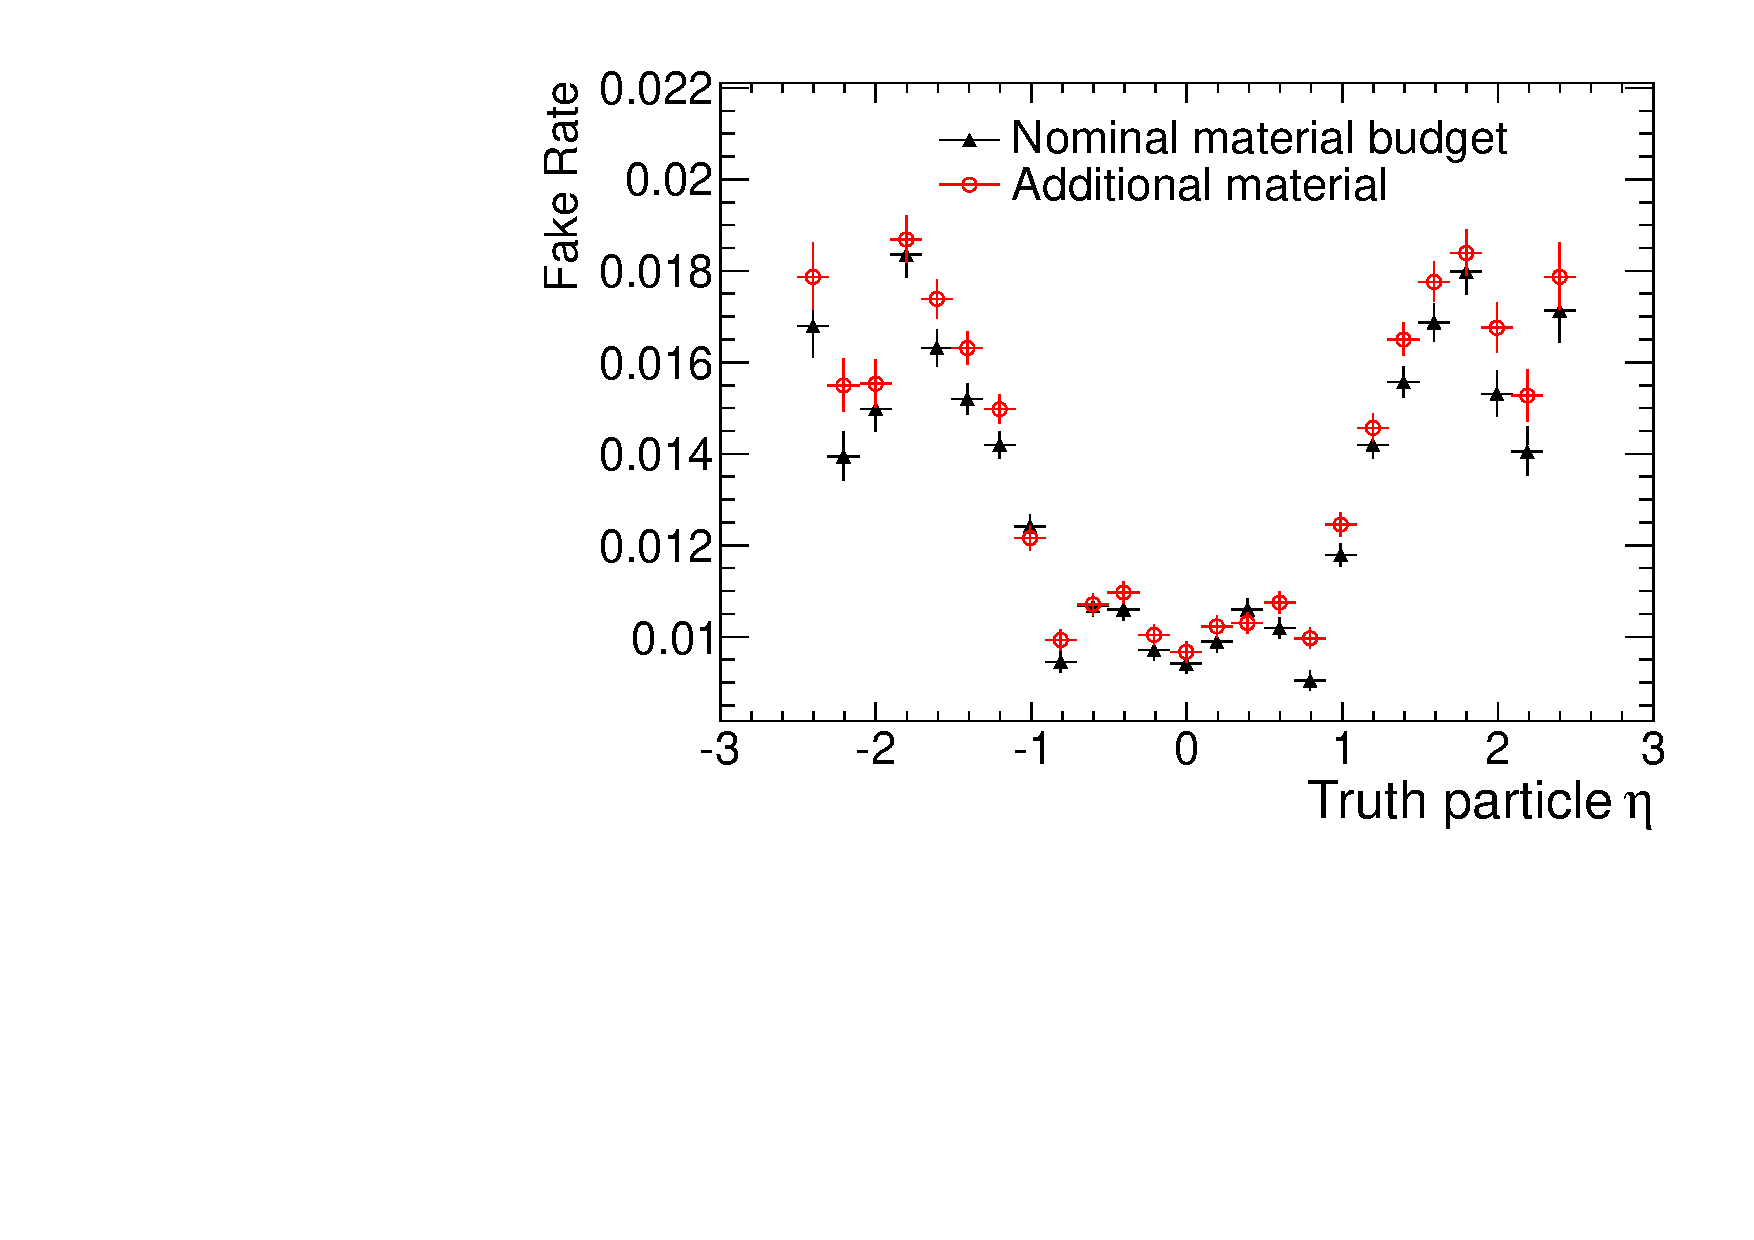
\includegraphics[width=0.7\textwidth]{figure/trackjet/trk_fake_distro_eta2.pdf}
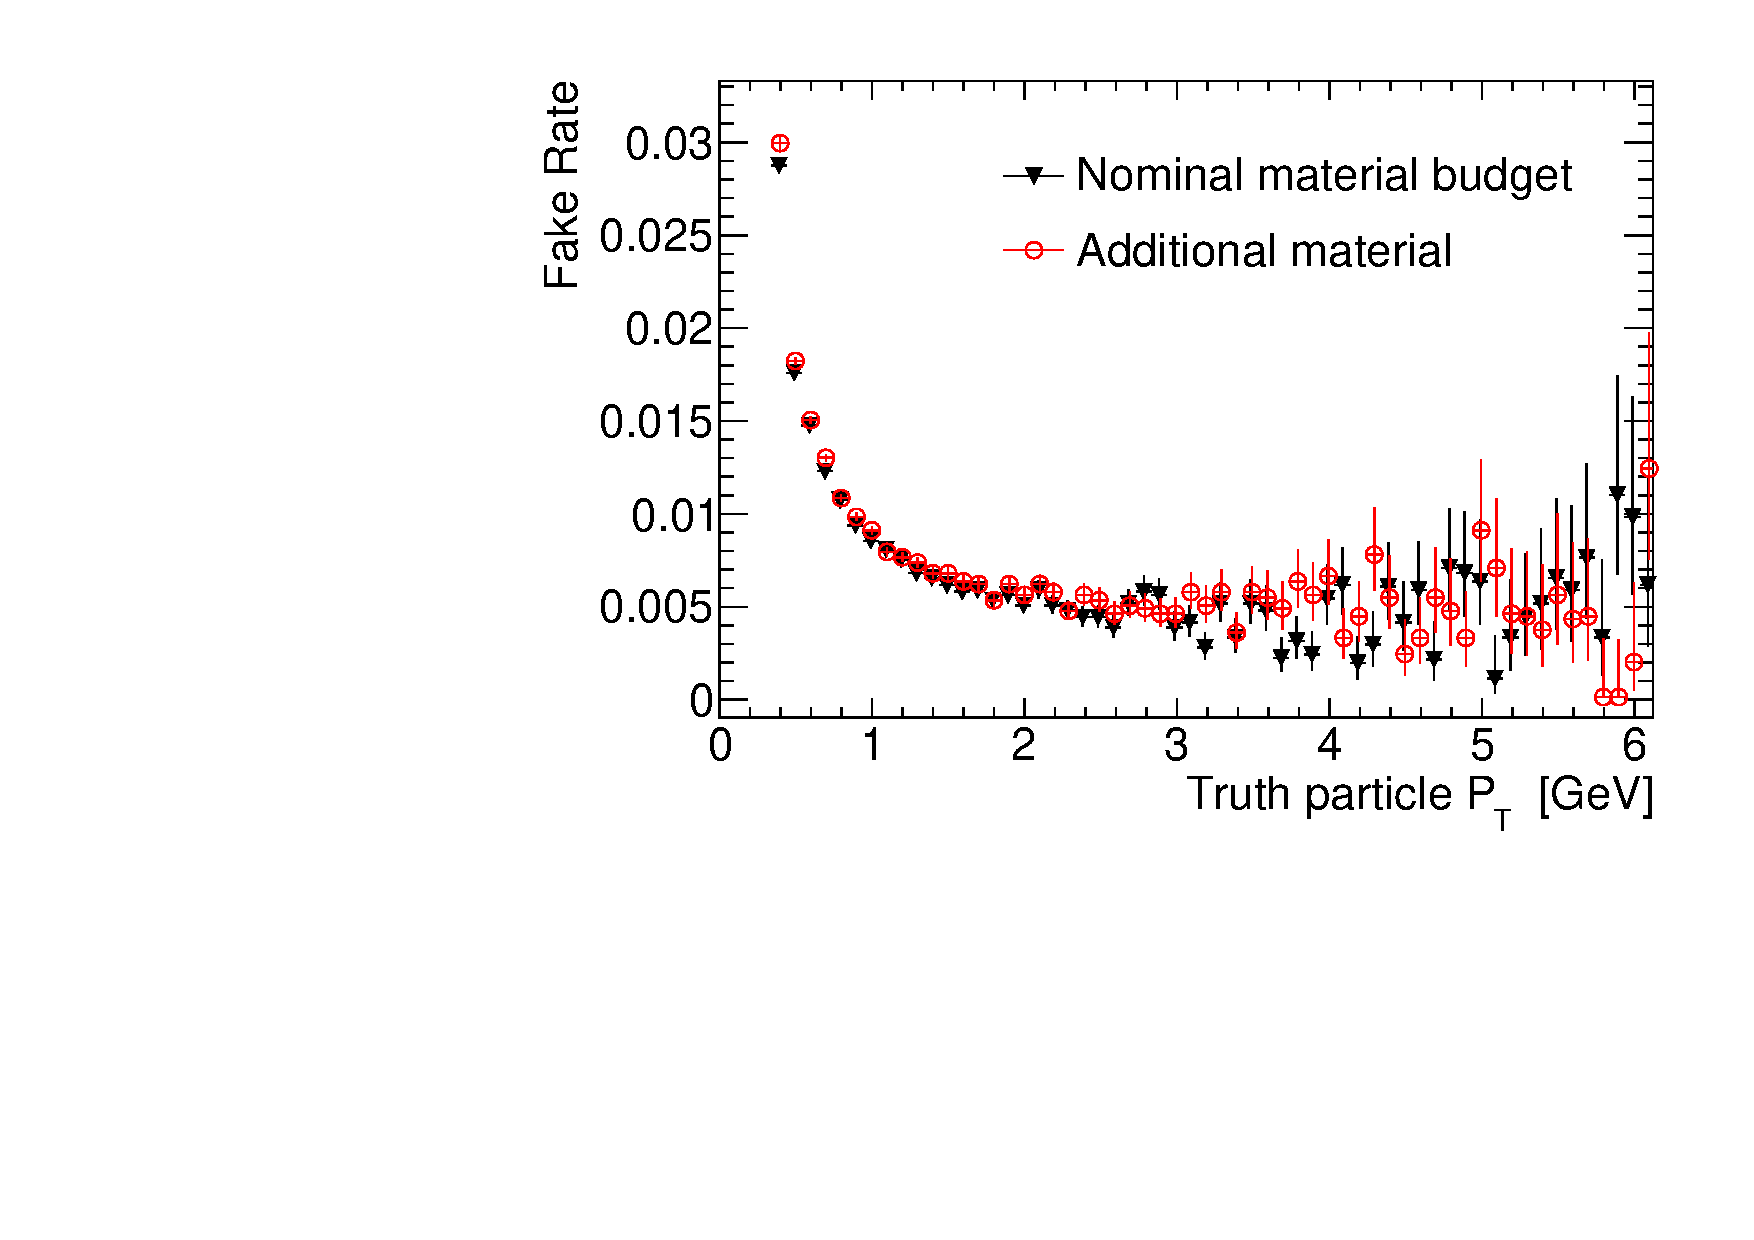
\includegraphics[width=0.7\textwidth]{figure/trackjet/fakerate_pt.pdf}
%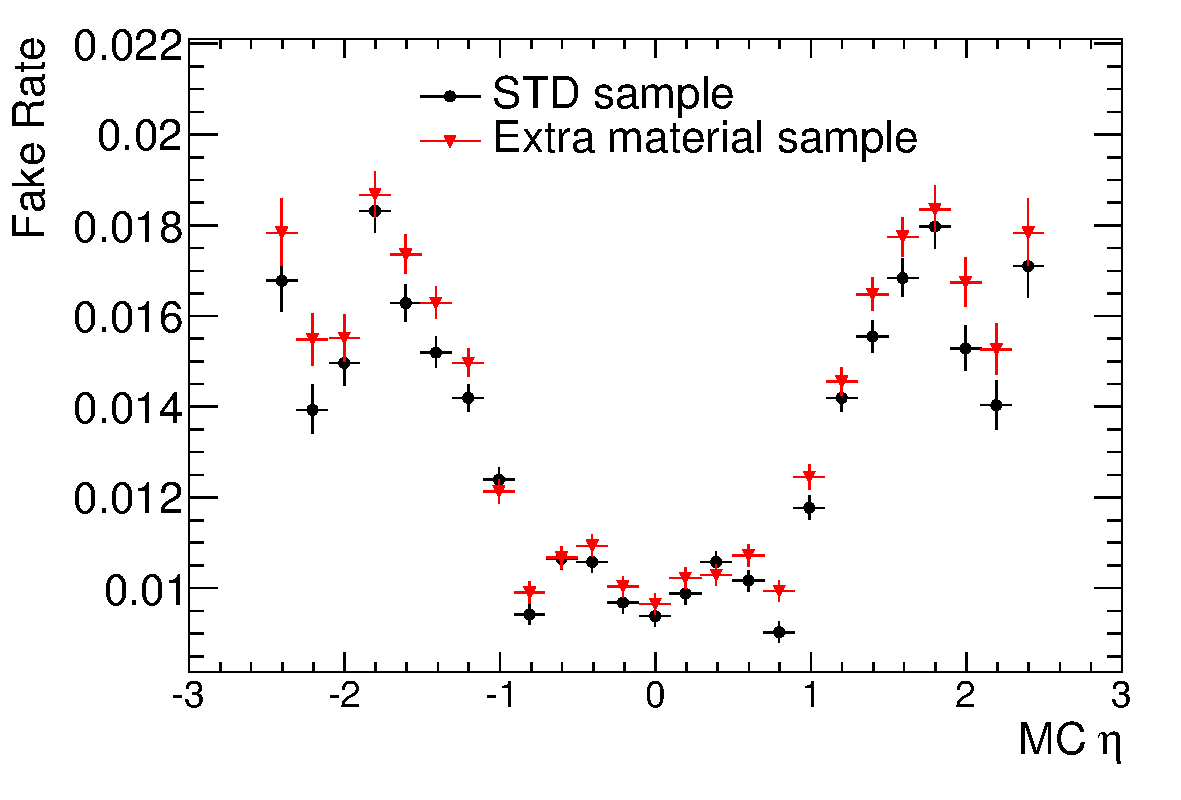
\includegraphics[width=0.45\textwidth]{figure/trackjet/T7/trk_fake_etauptade.pdf}
%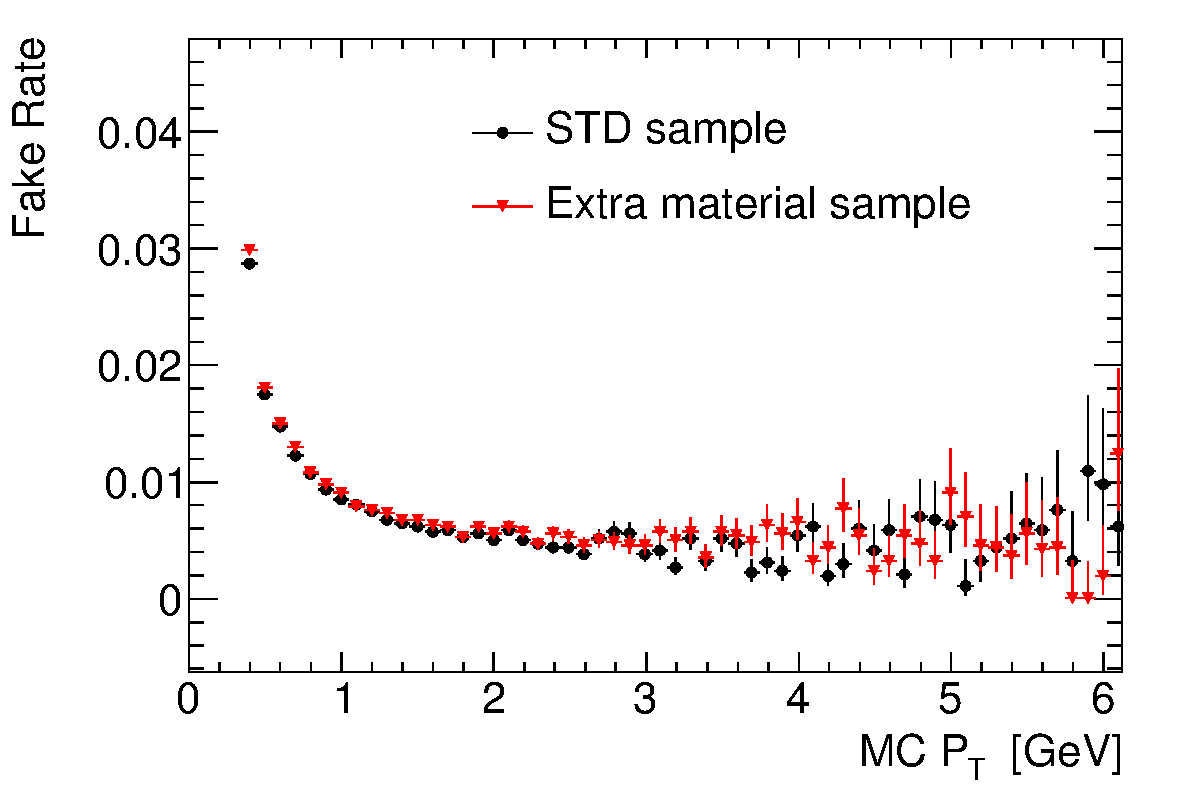
\includegraphics[width=0.45\textwidth]{figure/trackjet/T7/trk_fake_uptade.pdf}
\caption{Track fake rate as a function of the associated truth particle $\eta$ (left) and $\pt$ (right).
	The results are shown for the two simulated samples of of minimum bias processes, one with a nominal material budget
	and one with 10\%  additional inner detector material.}

\label{fig:trk_fakereate}
\end{figure}    

\begin{figure}[!tp]
\centering
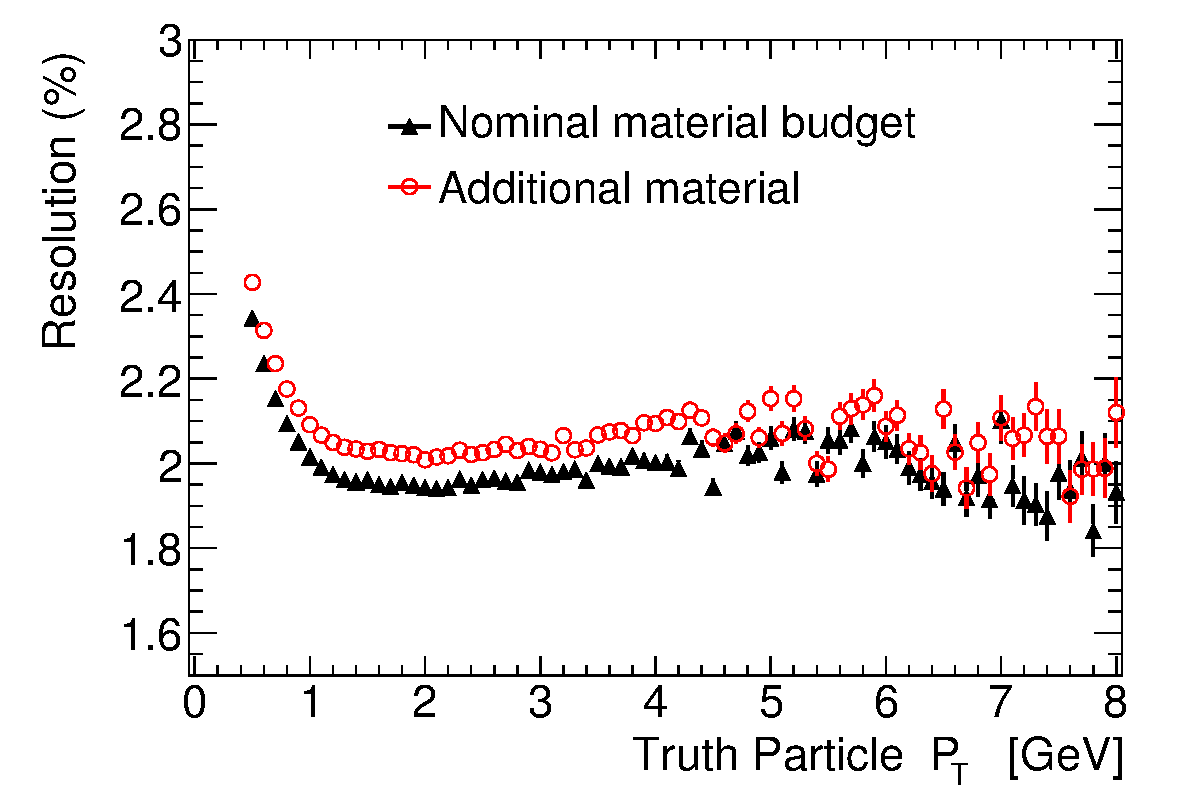
\includegraphics[width=0.7\textwidth]{figure/trackjet/resolution2.pdf}
%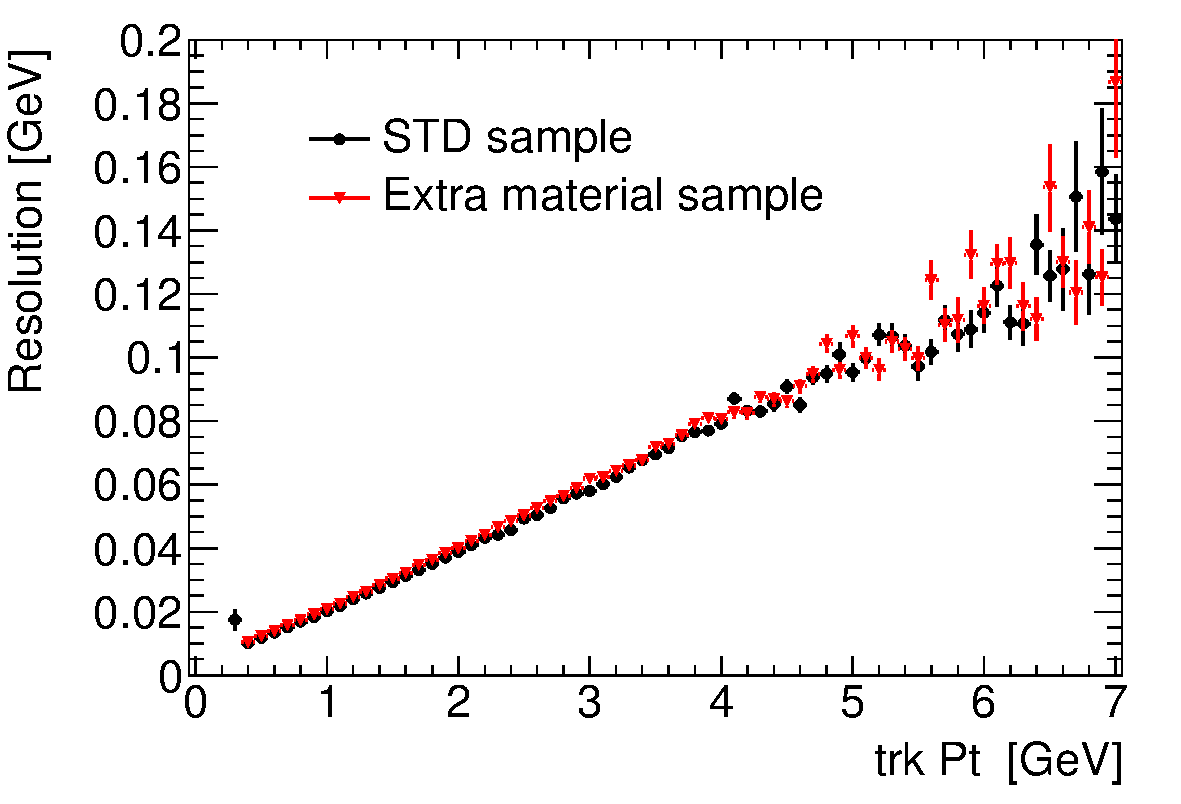
\includegraphics[width=0.6\textwidth]{figure/trackjet/T7/trk_reso_updater.pdf}
\caption{Track momentum resolution  relative to the matched truth particle as a function of truth particle $\pt$.
	The results are shown for the two simulated samples of of minimum bias processes, one with a nominal material budget
	and one with 10\%  additional inner detector material.}


\label{fig:trk_reso}
\end{figure}    

\begin{figure}[p]
\centering
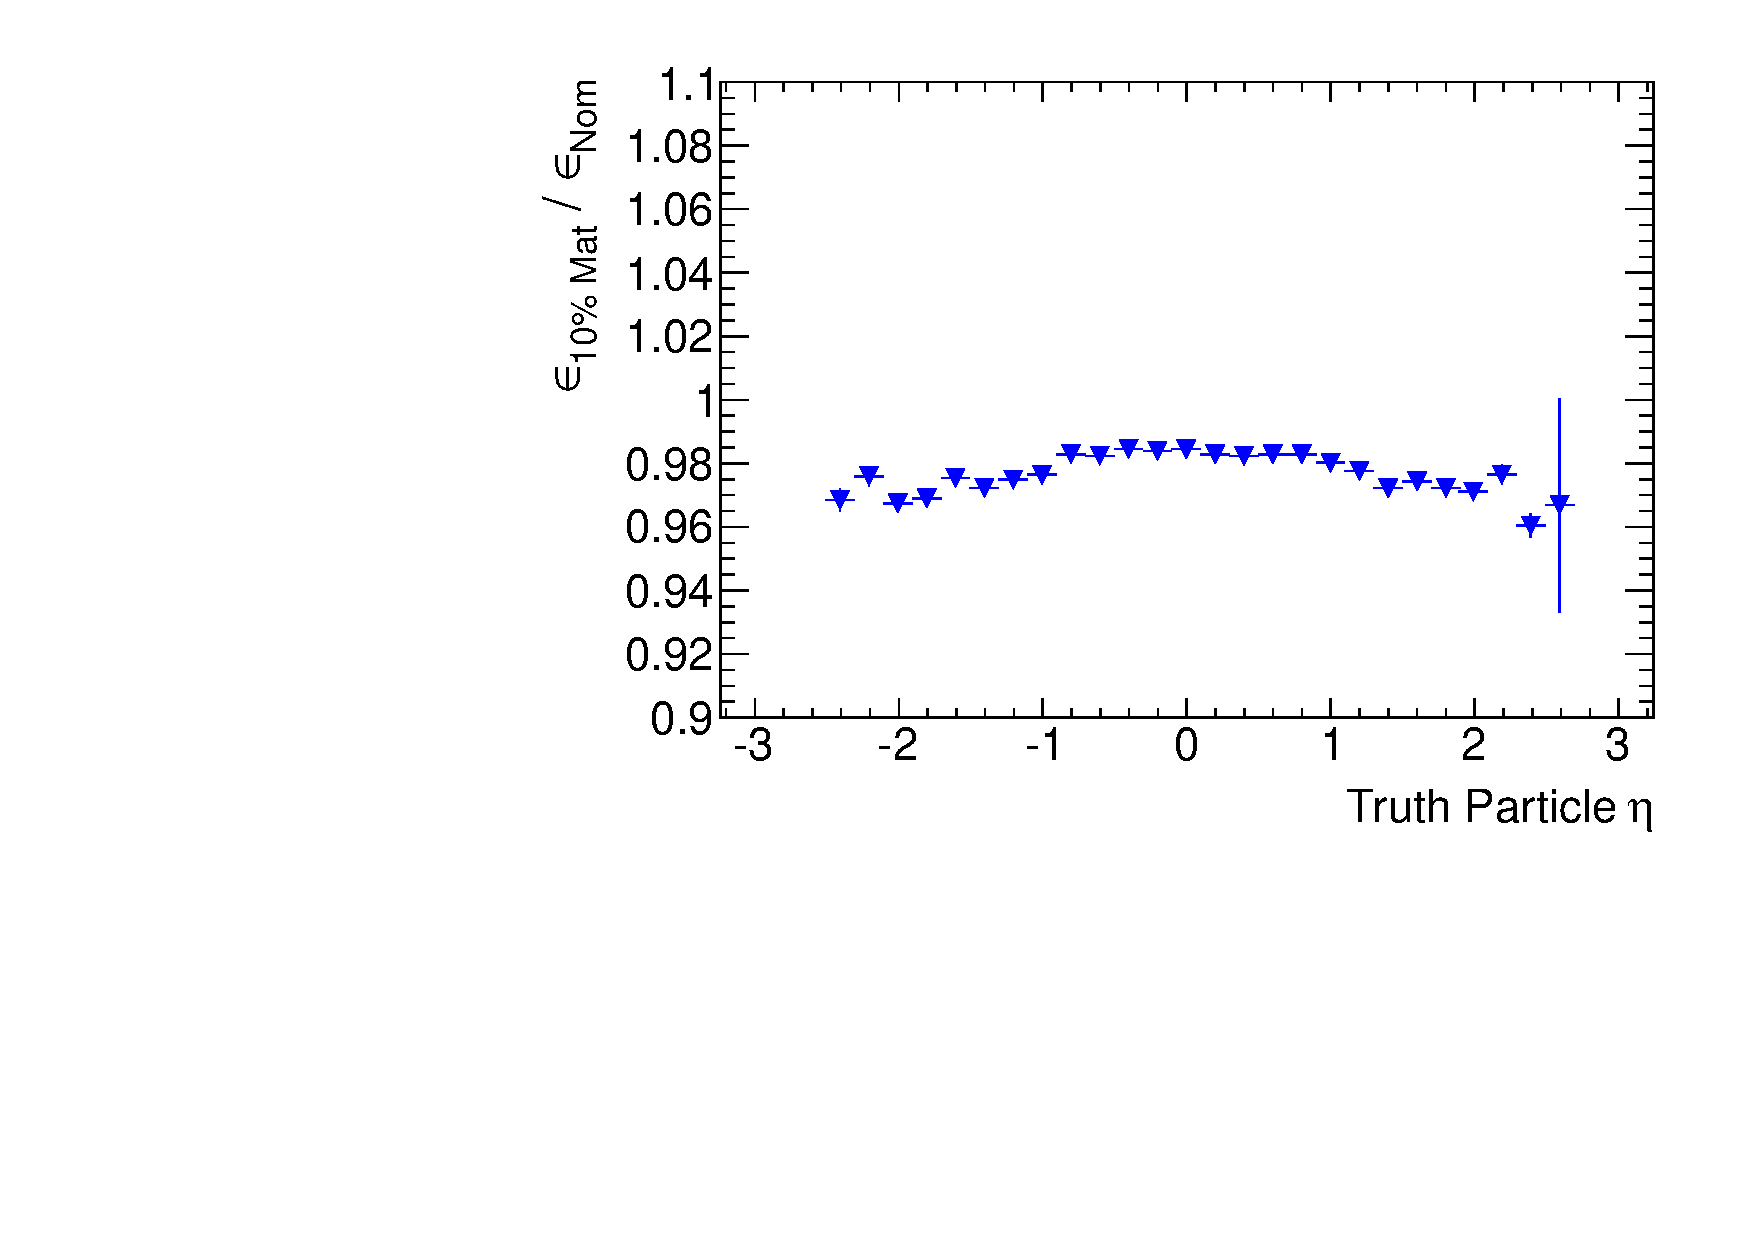
\includegraphics[width=0.7\textwidth]{figure/trackjet/trk_eff2.pdf}
%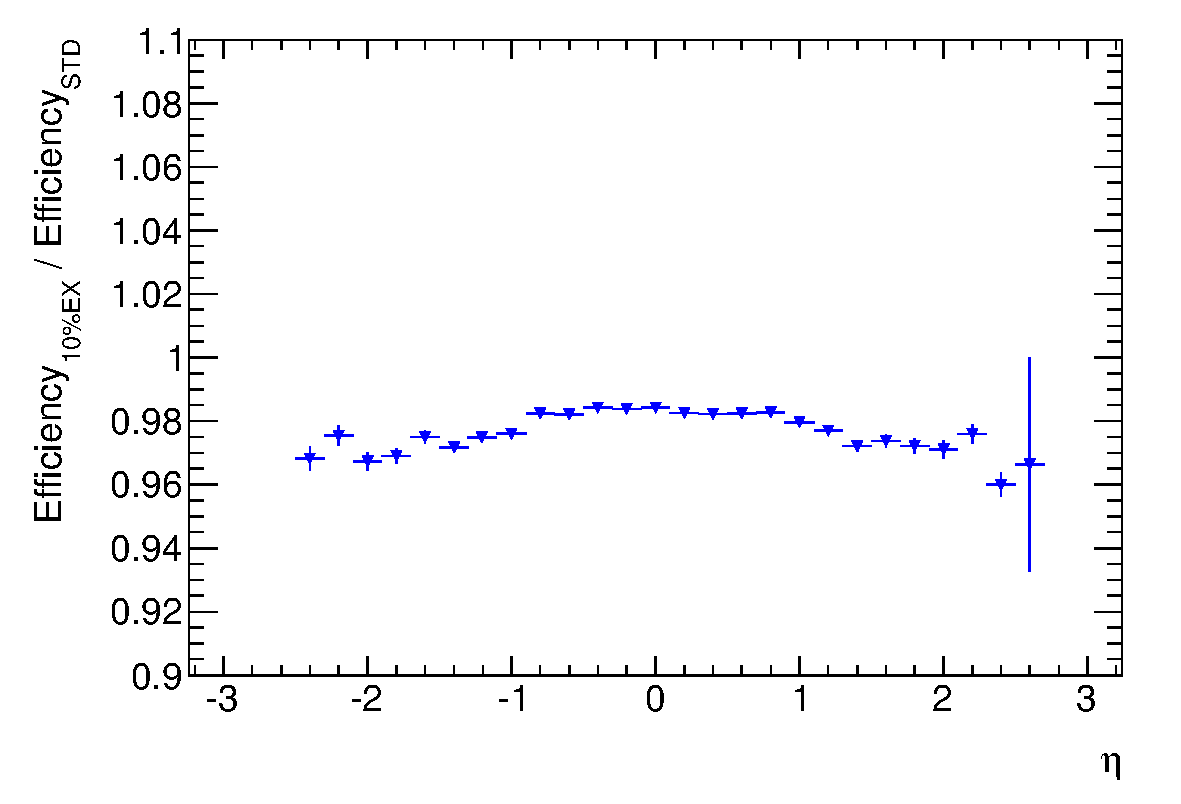
\includegraphics[width=0.6\textwidth]{figure/trackjet/T7/track_efficiency_ratio.pdf}
\caption{Ratio of track reconstruction efficiencies relative to primary truth particles as a function of truth particle $\eta$.
	 The ratio is shown for efficiency measured in minimum bias samples with the nominal material budget ($\epsilon_{Nom}$)
	and in the sample with 10\% of additional material ($\epsilon_{10\%Mat}$).}

\label{fig:trk_eff}
\end{figure}    


Reconstruction of inefficienct track-jets in a sample with nominal material budjet is also directly compared 
to the track-jets reconstruction in a sample with added additional ID material. Track-jet are mathced
to truth-jet (as described in section~\ref{sec:tj_perf}) in order to determine the track-jet 
reconstruction efficiency and energy scale, shown respectively in Figure~\ref{fig:tj10tjex_eff} and~\ref{fig:tj10tjex_pt}$\,$.
Inefficient track-jets reproduce correctly the impact  of additional material,
giving in most of the cases a conservative estimate of the corresponding systematic uncertainties.


\begin{figure}[tp]
\centering
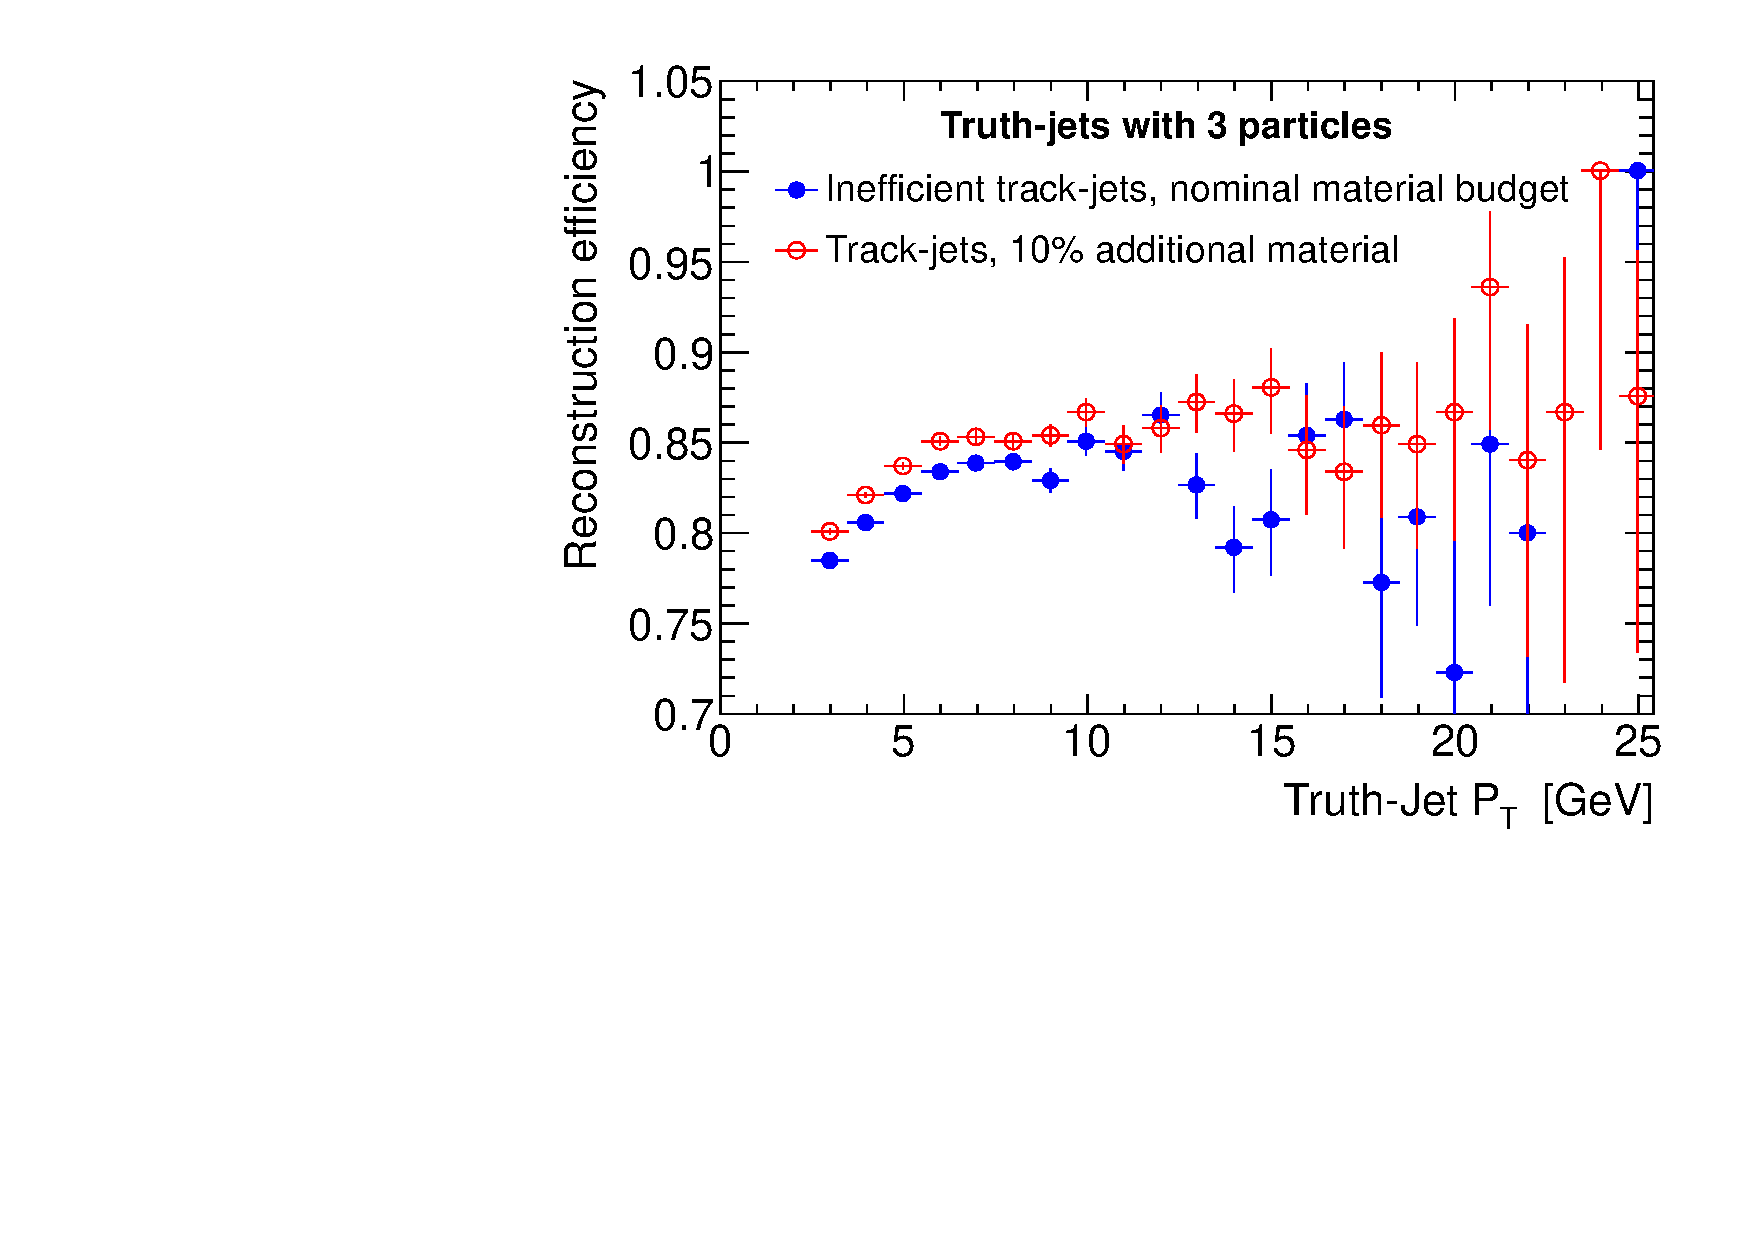
\includegraphics[width=0.60\textwidth]{figure/trackjet/T7/inef_10cent_eff_3S.pdf}
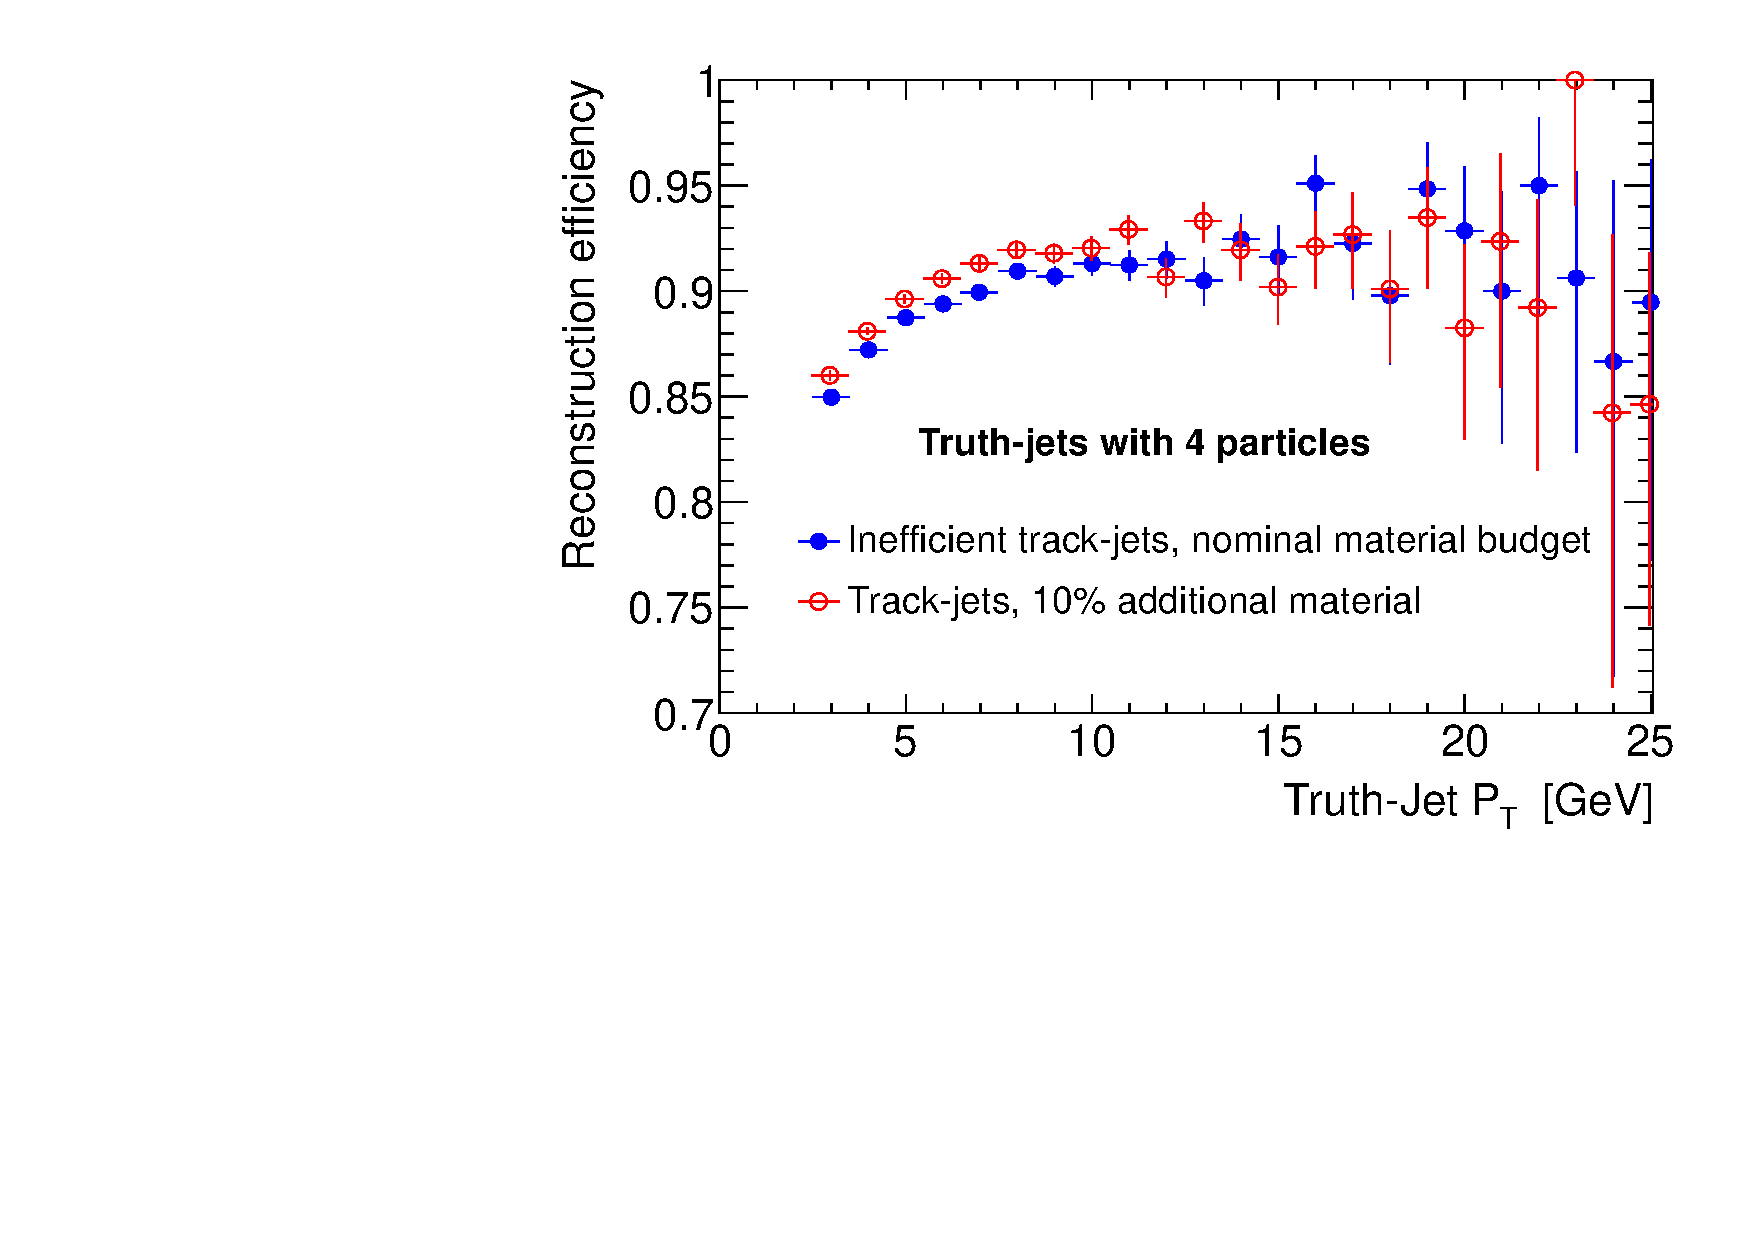
\includegraphics[width=0.60\textwidth]{figure/trackjet/T7/inef_10cent_eff_4S.pdf}
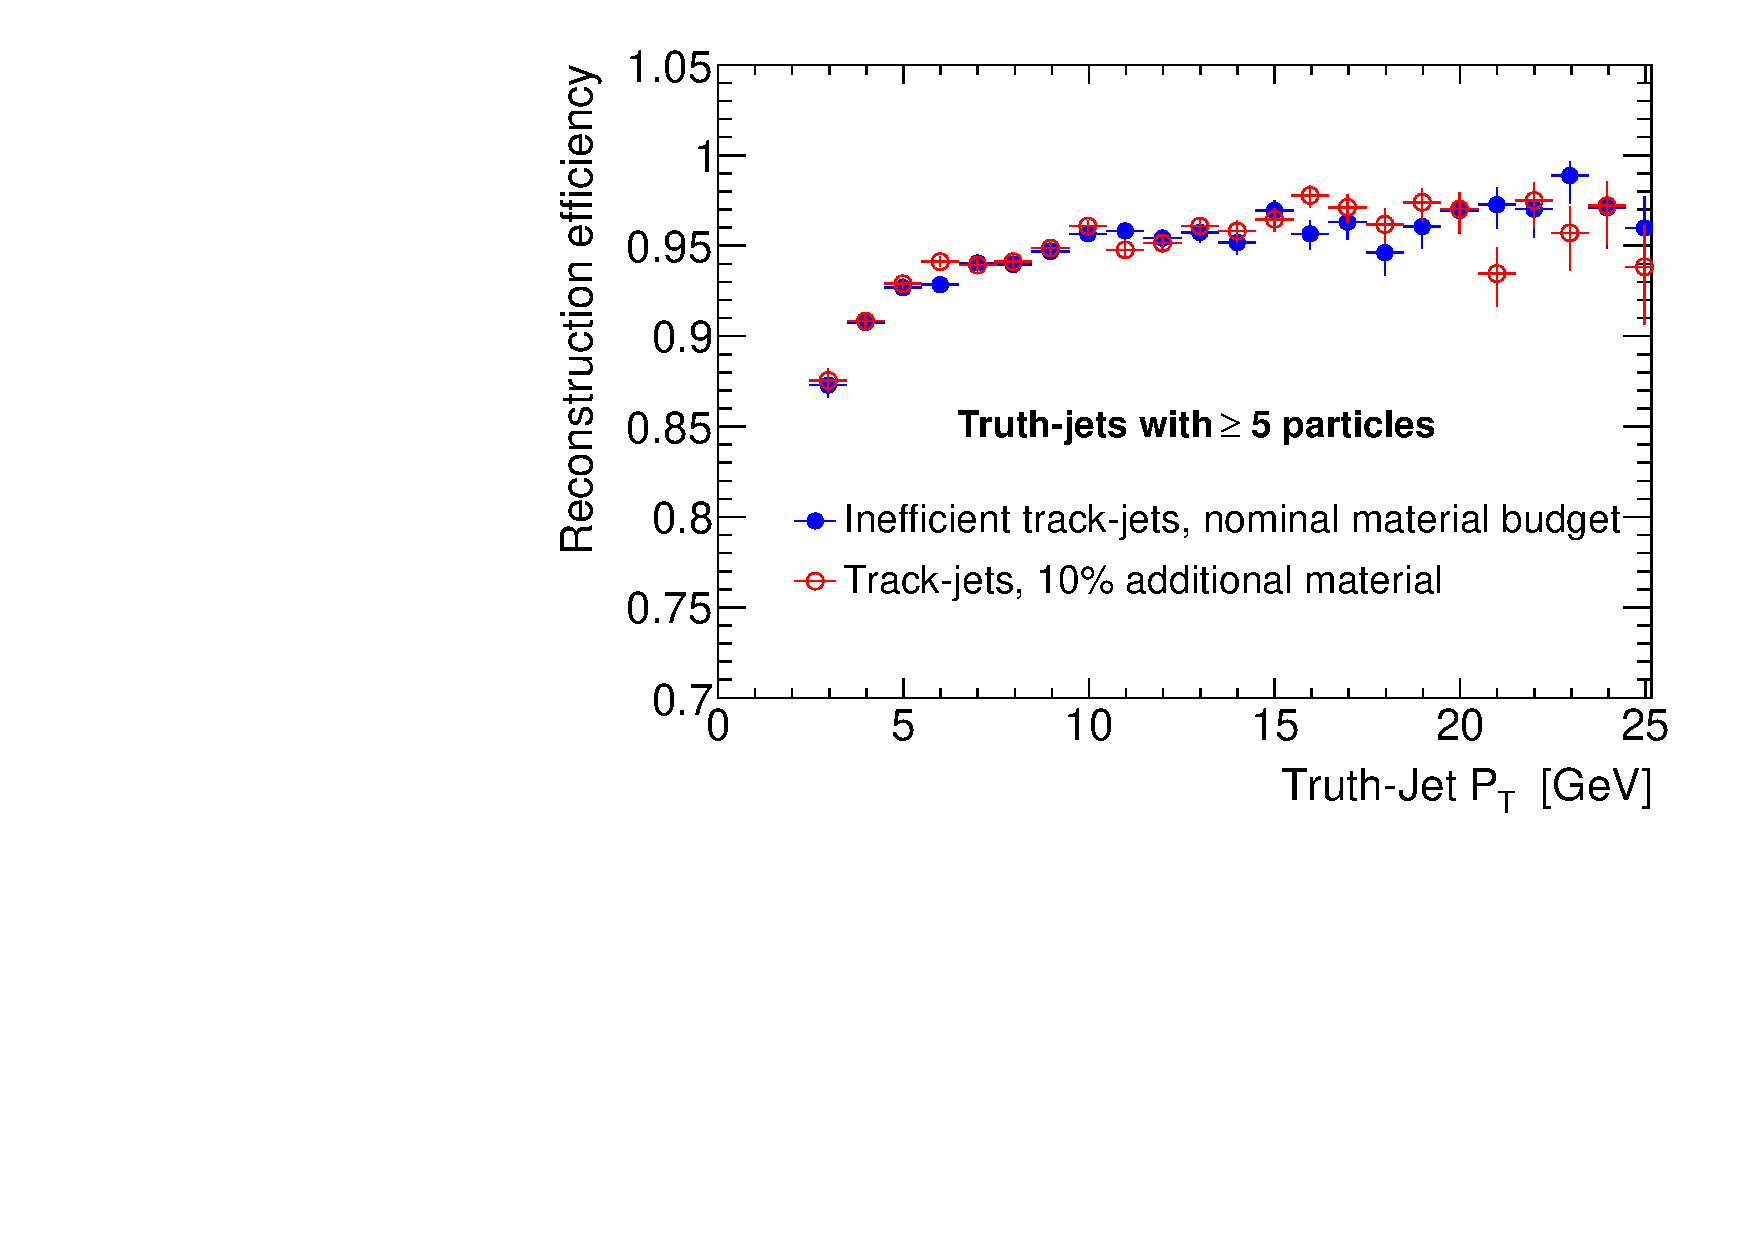
\includegraphics[width=0.60\textwidth]{figure/trackjet/T7/inef_10cent_eff_5S.pdf}
\caption{Jet reconstruction efficiency relative to truth-jet for inefficient track-jets reconstructed in a minimum bias 
	sample with nominal material budget and for the nominal track-jet reconstruction in a sample with 10\% additional material.
	Result are shown separately for truth-jet consisting of 3,4 and $\geq 5$ truth particle.}

\label{fig:tj10tjex_eff}
\end{figure}    

\begin{figure}[tp]
\centering
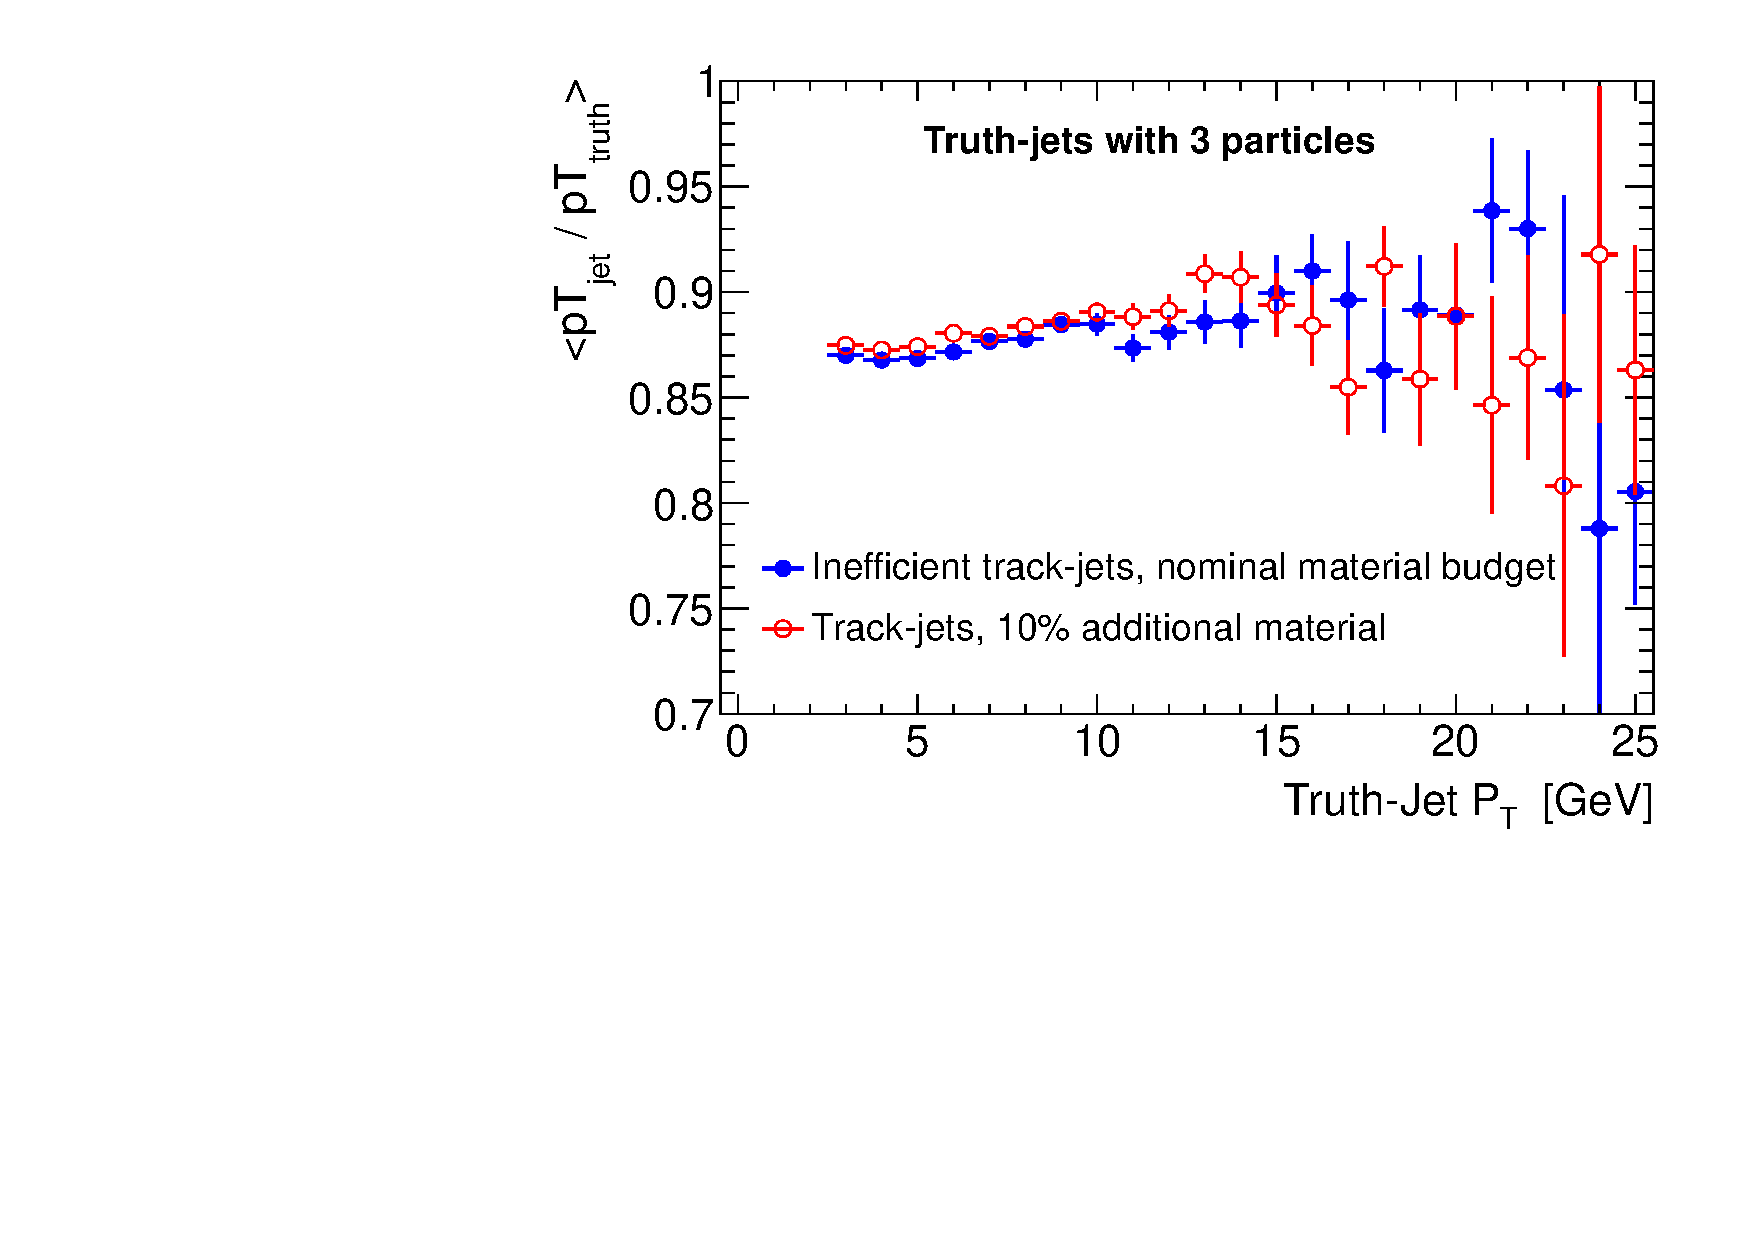
\includegraphics[width=0.60\textwidth]{figure/trackjet/T7/inef_10cent_pt_3S.pdf}
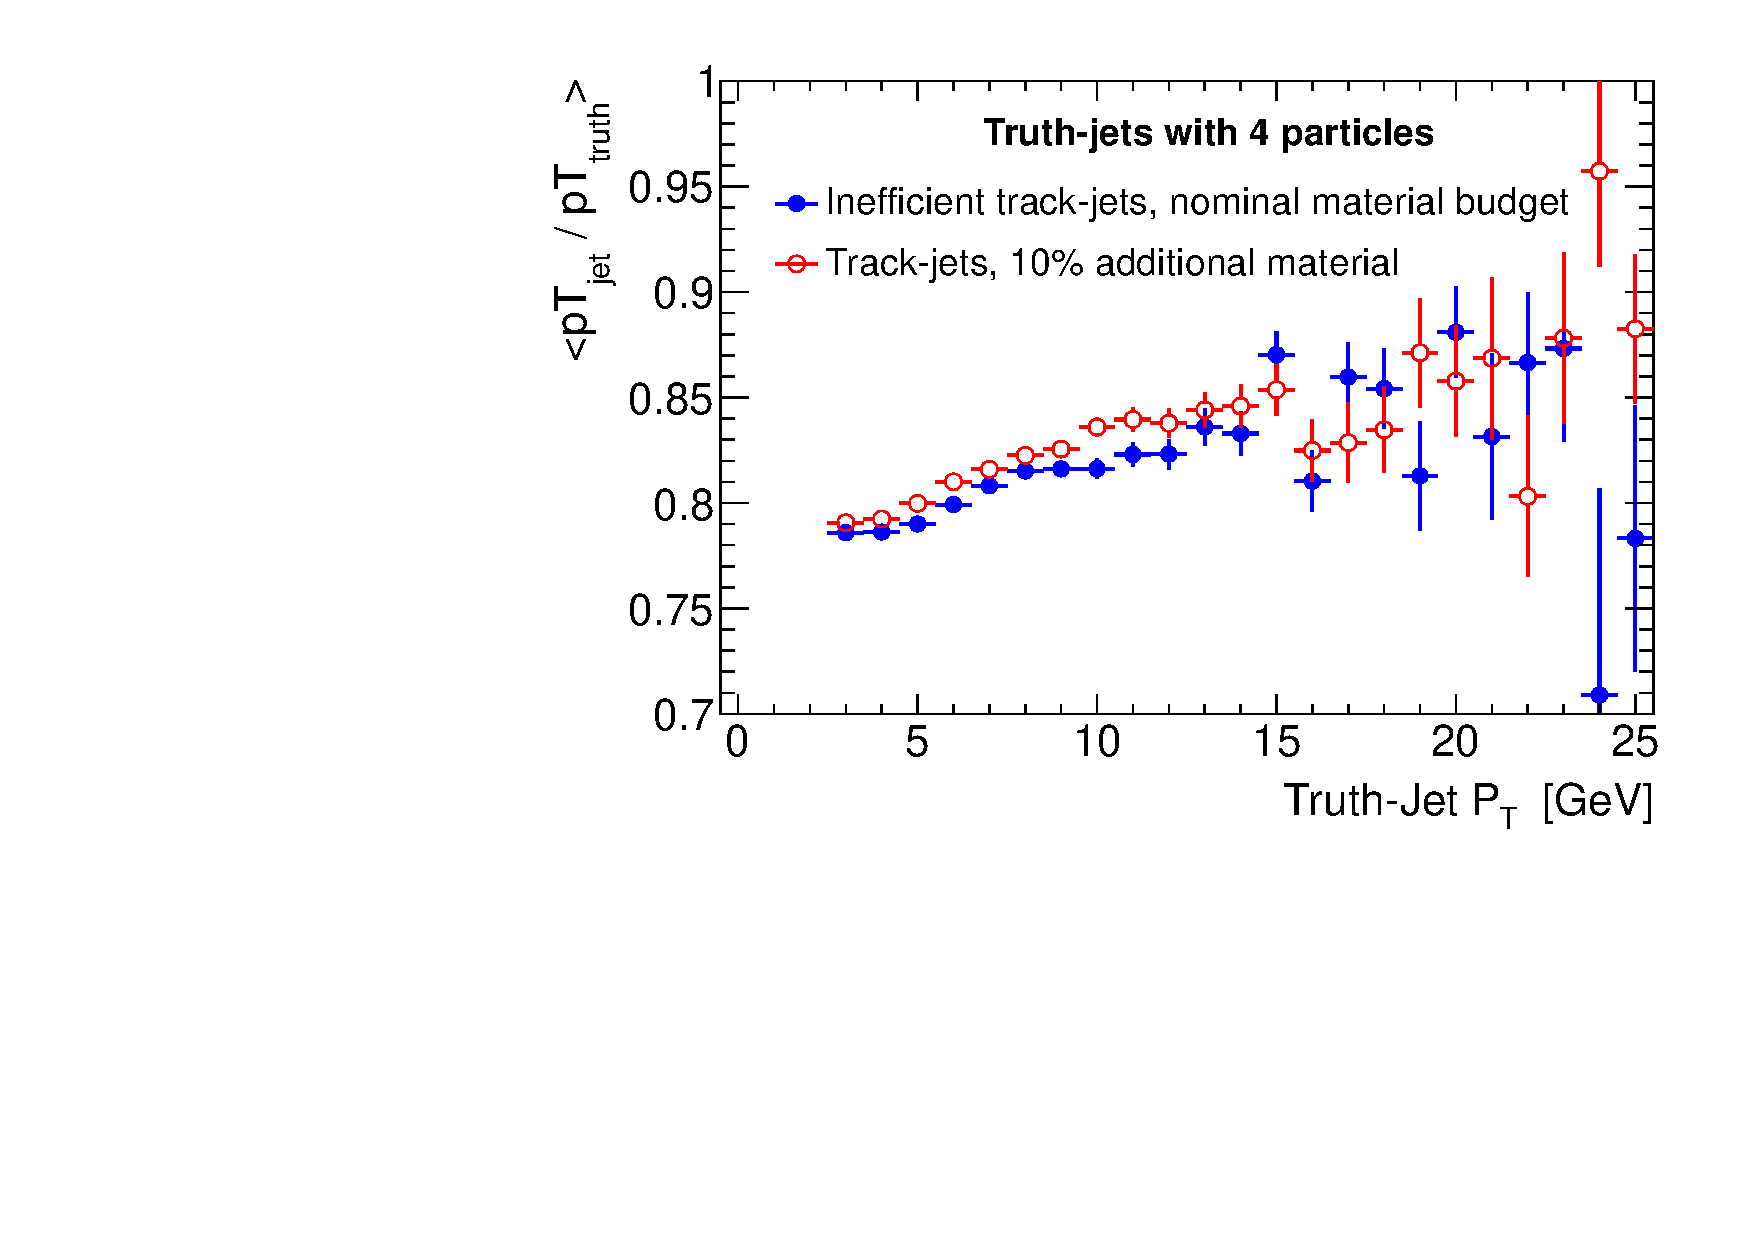
\includegraphics[width=0.60\textwidth]{figure/trackjet/T7/inef_10cent_pt_4S.pdf}
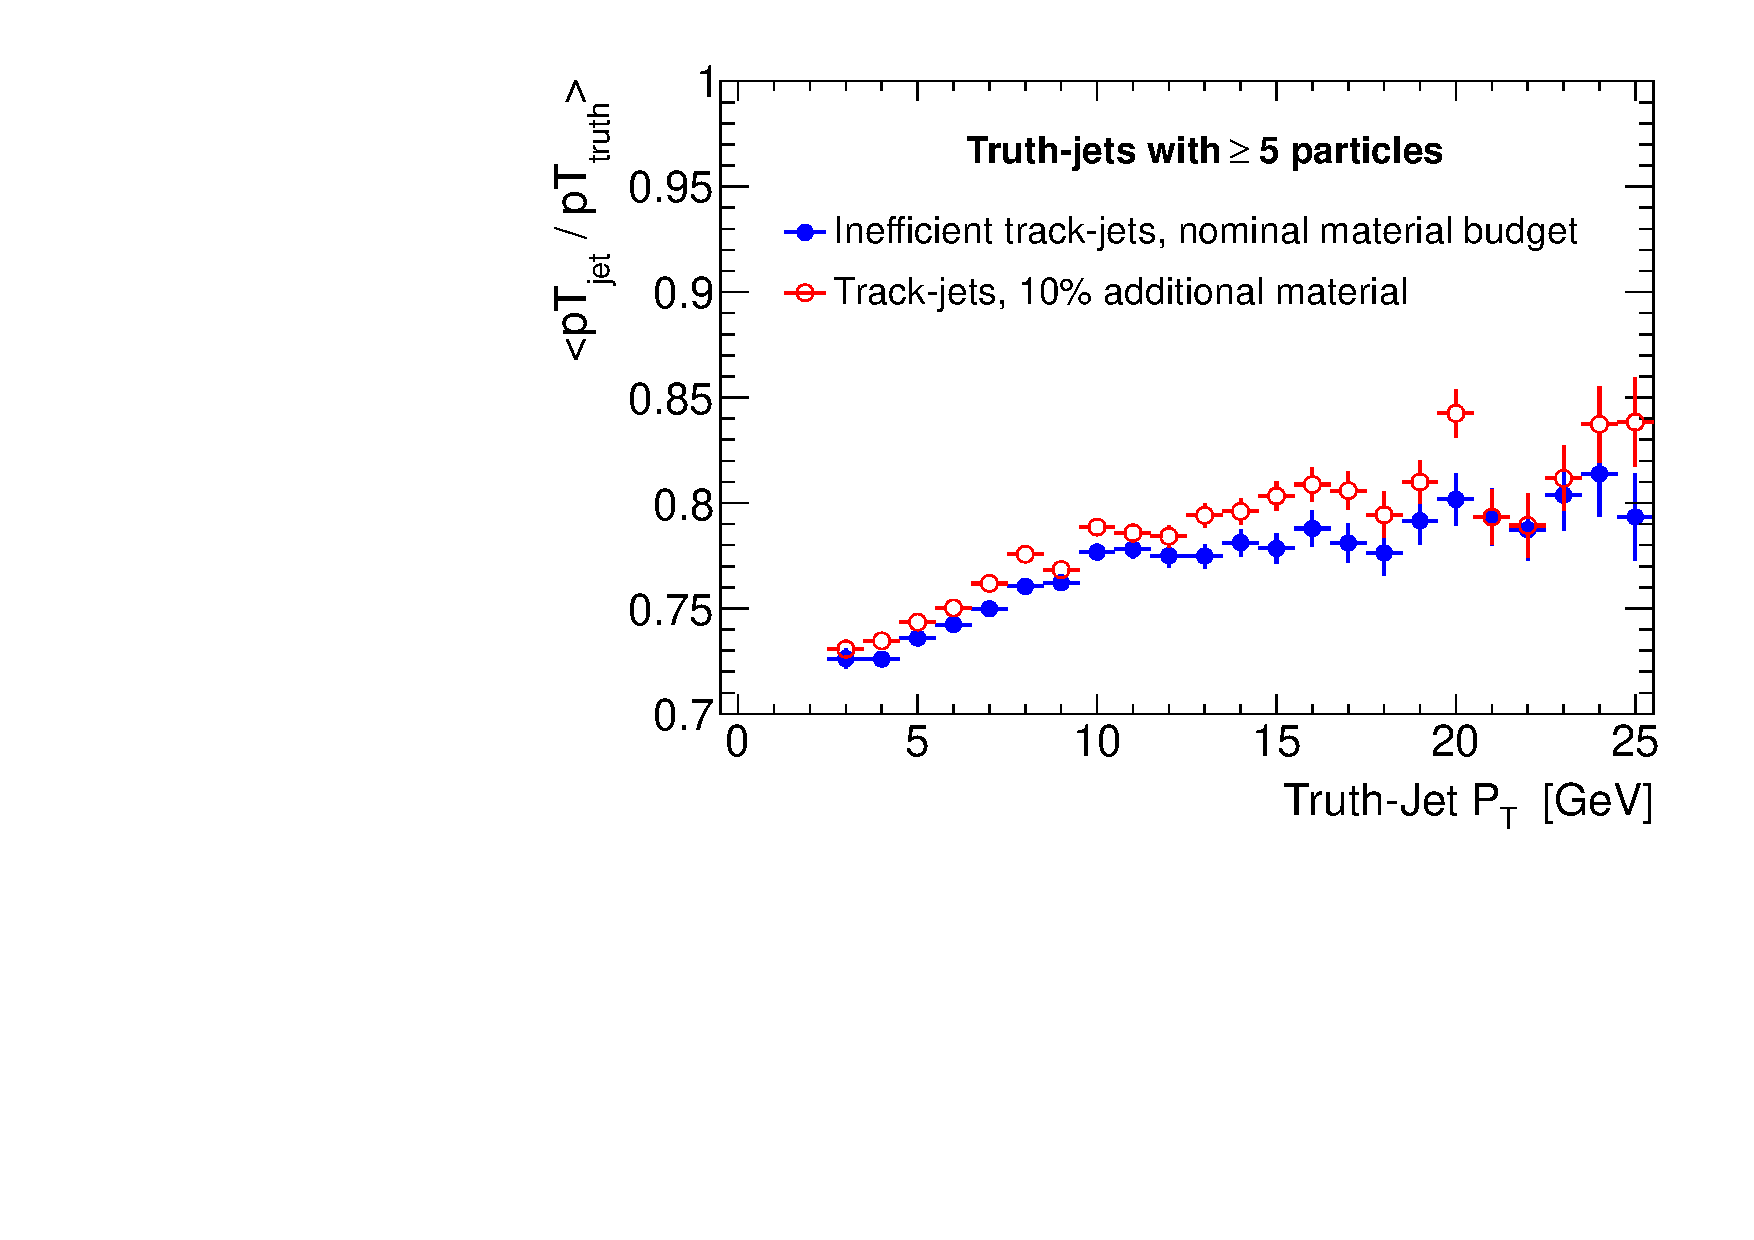
\includegraphics[width=0.60\textwidth]{figure/trackjet/T7/inef_10cent_pt_5S.pdf}
\caption{Fraction of the jet transverse momentum relative to truth-jet transverse momentum shown for 
	 inefficient track-jets reconstructed in a minimum bias 
	sample with nominal material budget and for the nominal track-jet reconstruction in a sample with 10\% additional material.
	Result are shown separately for truth-jet consisting of 3,4 and $\geq 5$ truth particle.}

\label{fig:tj10tjex_pt}
\end{figure}    
























